% ***********************************************
\chapter{Preliminaries}\label{ch:preliminaries}
% ***********************************************

% ***********************************************
\section{Coxeter Groups}
% ***********************************************

First of all, we define the main object of interest we want to study.

\begin{definition}\label{def:CoxeterGroup}
    Let \(S\) be a set consisting of elements \(s_i\) indexed by an index set \(I\) with \(\abs{I} = n < \infty\).
    Let  \((m_{ij}) = M\) be a symmetrical matrix in \((\N\cup\{\infty\})^{n\times n}\), where \(m_{ii}=1\) for all \(i\) and \(m_{ij}\geq 2\) for \(i\neq j\).
    Define a group \(W\) via the following presentation:
    \begin{equation*}
        W := \groupp{S}{(s_is_j)^{m_{ij}}=1 \; \text{for all} \; i,j\in I},
    \end{equation*}
    where the relations with \(m_{ij} = \infty\) are usually ommited, i.e. give trivial relations.
    The pair \((W, S)\) is called a \emph{Coxeter System} and \(M\) is called the corresponding \emph{Coxeter Matrix}.
    A \emph{Coxeter group} is a group isomorphic to a group \(W\), corresponding to a Coxeter System \((W,S)\).
    It is generated by the set \(S\).
\end{definition}

In this work we will be particularly interested in a special class of Coxeter groups that we call right-angled.
They are defined as follows, by imposing significant constraints on the entries of the Coxeter matrix.

\begin{definition}
    A Coxeter System \((W, S)\) is \emph{right-angled} if, for all distinct \(i,j\in I\), the condition \(m_{ij}\in\{2,\infty\}\) is satisfied.
    In this context, the group \(W\) is then called a \emph{right-angled Coxeter group (RACG)}.
\end{definition}

We give some important examples of Coxeter groups as well as right-angled Coxeter groups.

\begin{example}
    \begin{enumerate}\label{ex:freeprod}
        \item Dihedral groups, \(D_{2m} \cong \groupp{s_1, s_2}{s_1^2 = s_2^2 = 1, (s_1s_2)^m = 1}\) are Coxeter groups for all \(m\in\N\).
        \item The triangle groups, \(\Delta(l,m,n) \cong \groupp{r,s,t}{r^2 = s^2 = t^2 = (rs)^l = (st)^m = (tr)^n = 1}\) \\
              with \(l, m\) and \(n\) integers greater or equal to \(2\) are Coxeter groups.
        \item The infinite Dihedral group, \(D_\infty \cong \groupp{s,t}{s^2=t^2=1}\) is a right-angled Coxeter group.
        \item The free product, \(\faktor{\Z}{2\Z}\ast\faktor{\Z}{2\Z}\ast\faktor{\Z}{2\Z} \cong \groupp{r,s,t}{r^2=s^2=t^2=1}\) is a right-angled Coxeter group.
    \end{enumerate}
\end{example}

In \Cref{fig:cayleygraphs} below, a small portion of the combinatorial Cayley graphs of these examples are depicted.
\newpage

\begin{figure}[ht]
    \caption{The combinatorial Cayley graph of ...}
    \label{fig:cayleygraphs}
    
    \centering
    \subfloat[\centering \(D_6\)]{{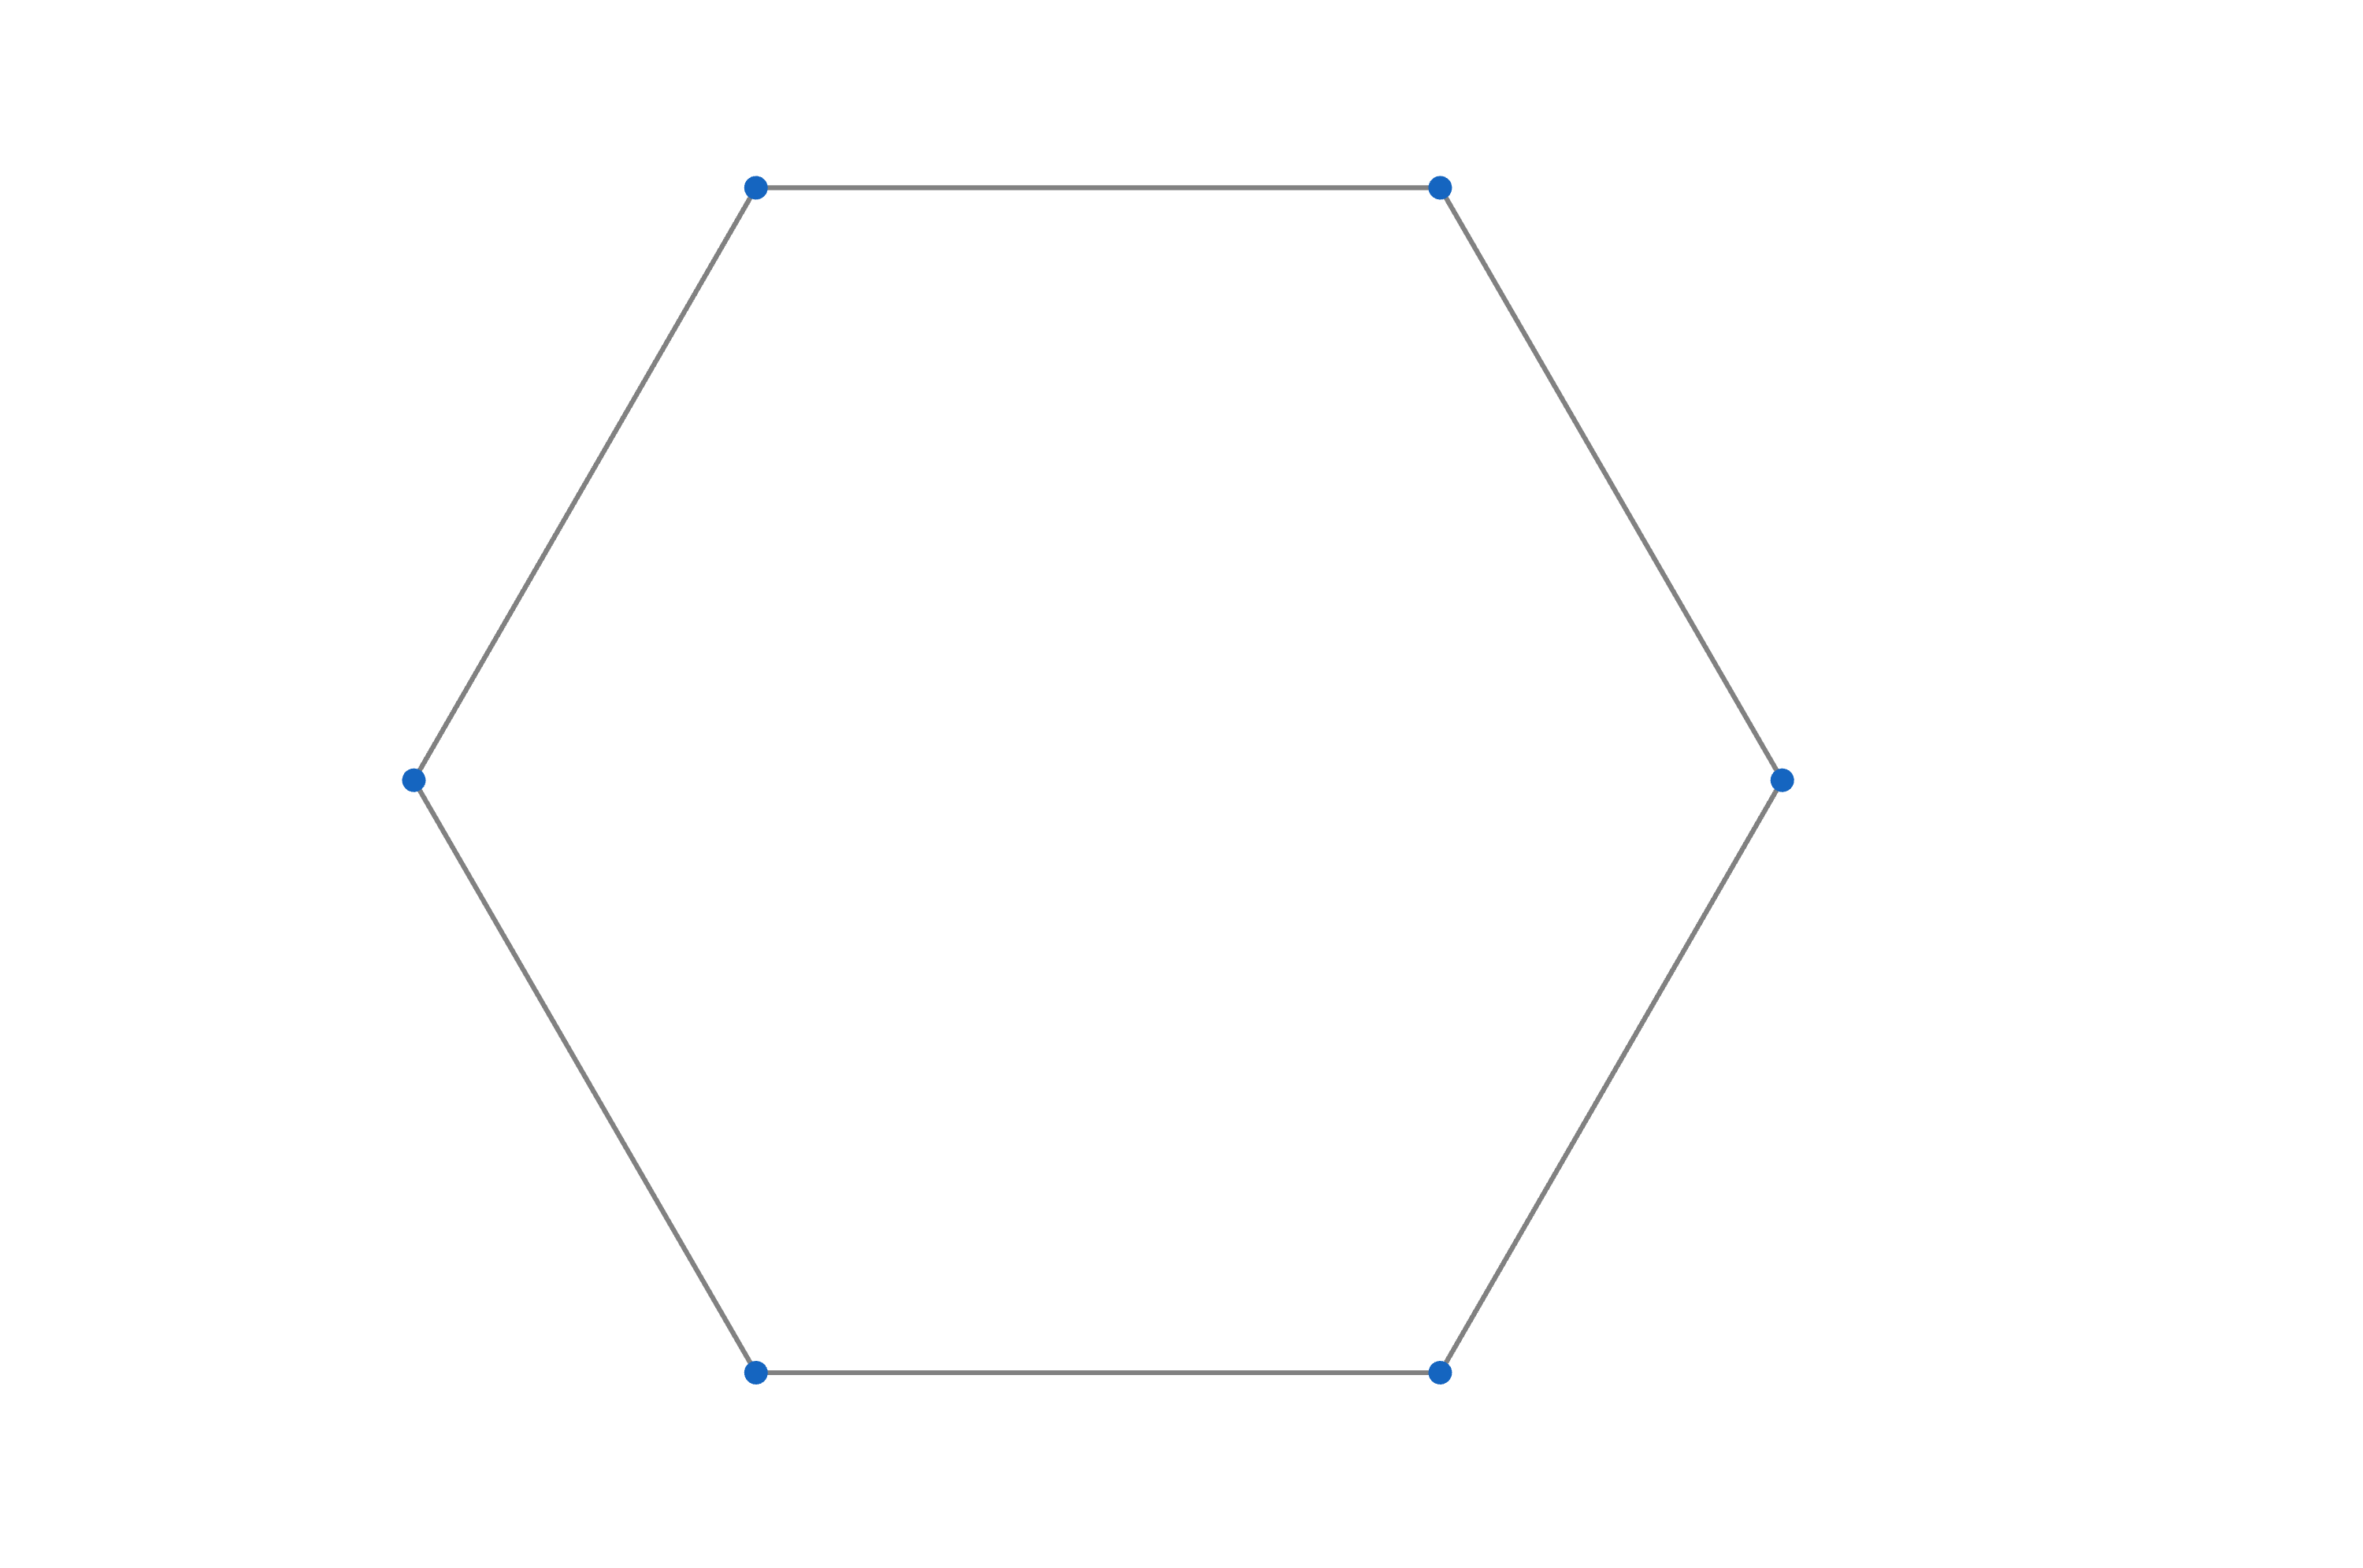
\includegraphics[width=4cm]{gfx/dihedral group cayley graph.png}}\label{img:dihedralcg}}
    \subfloat[\centering \(\Delta (3,3,3)\)]{{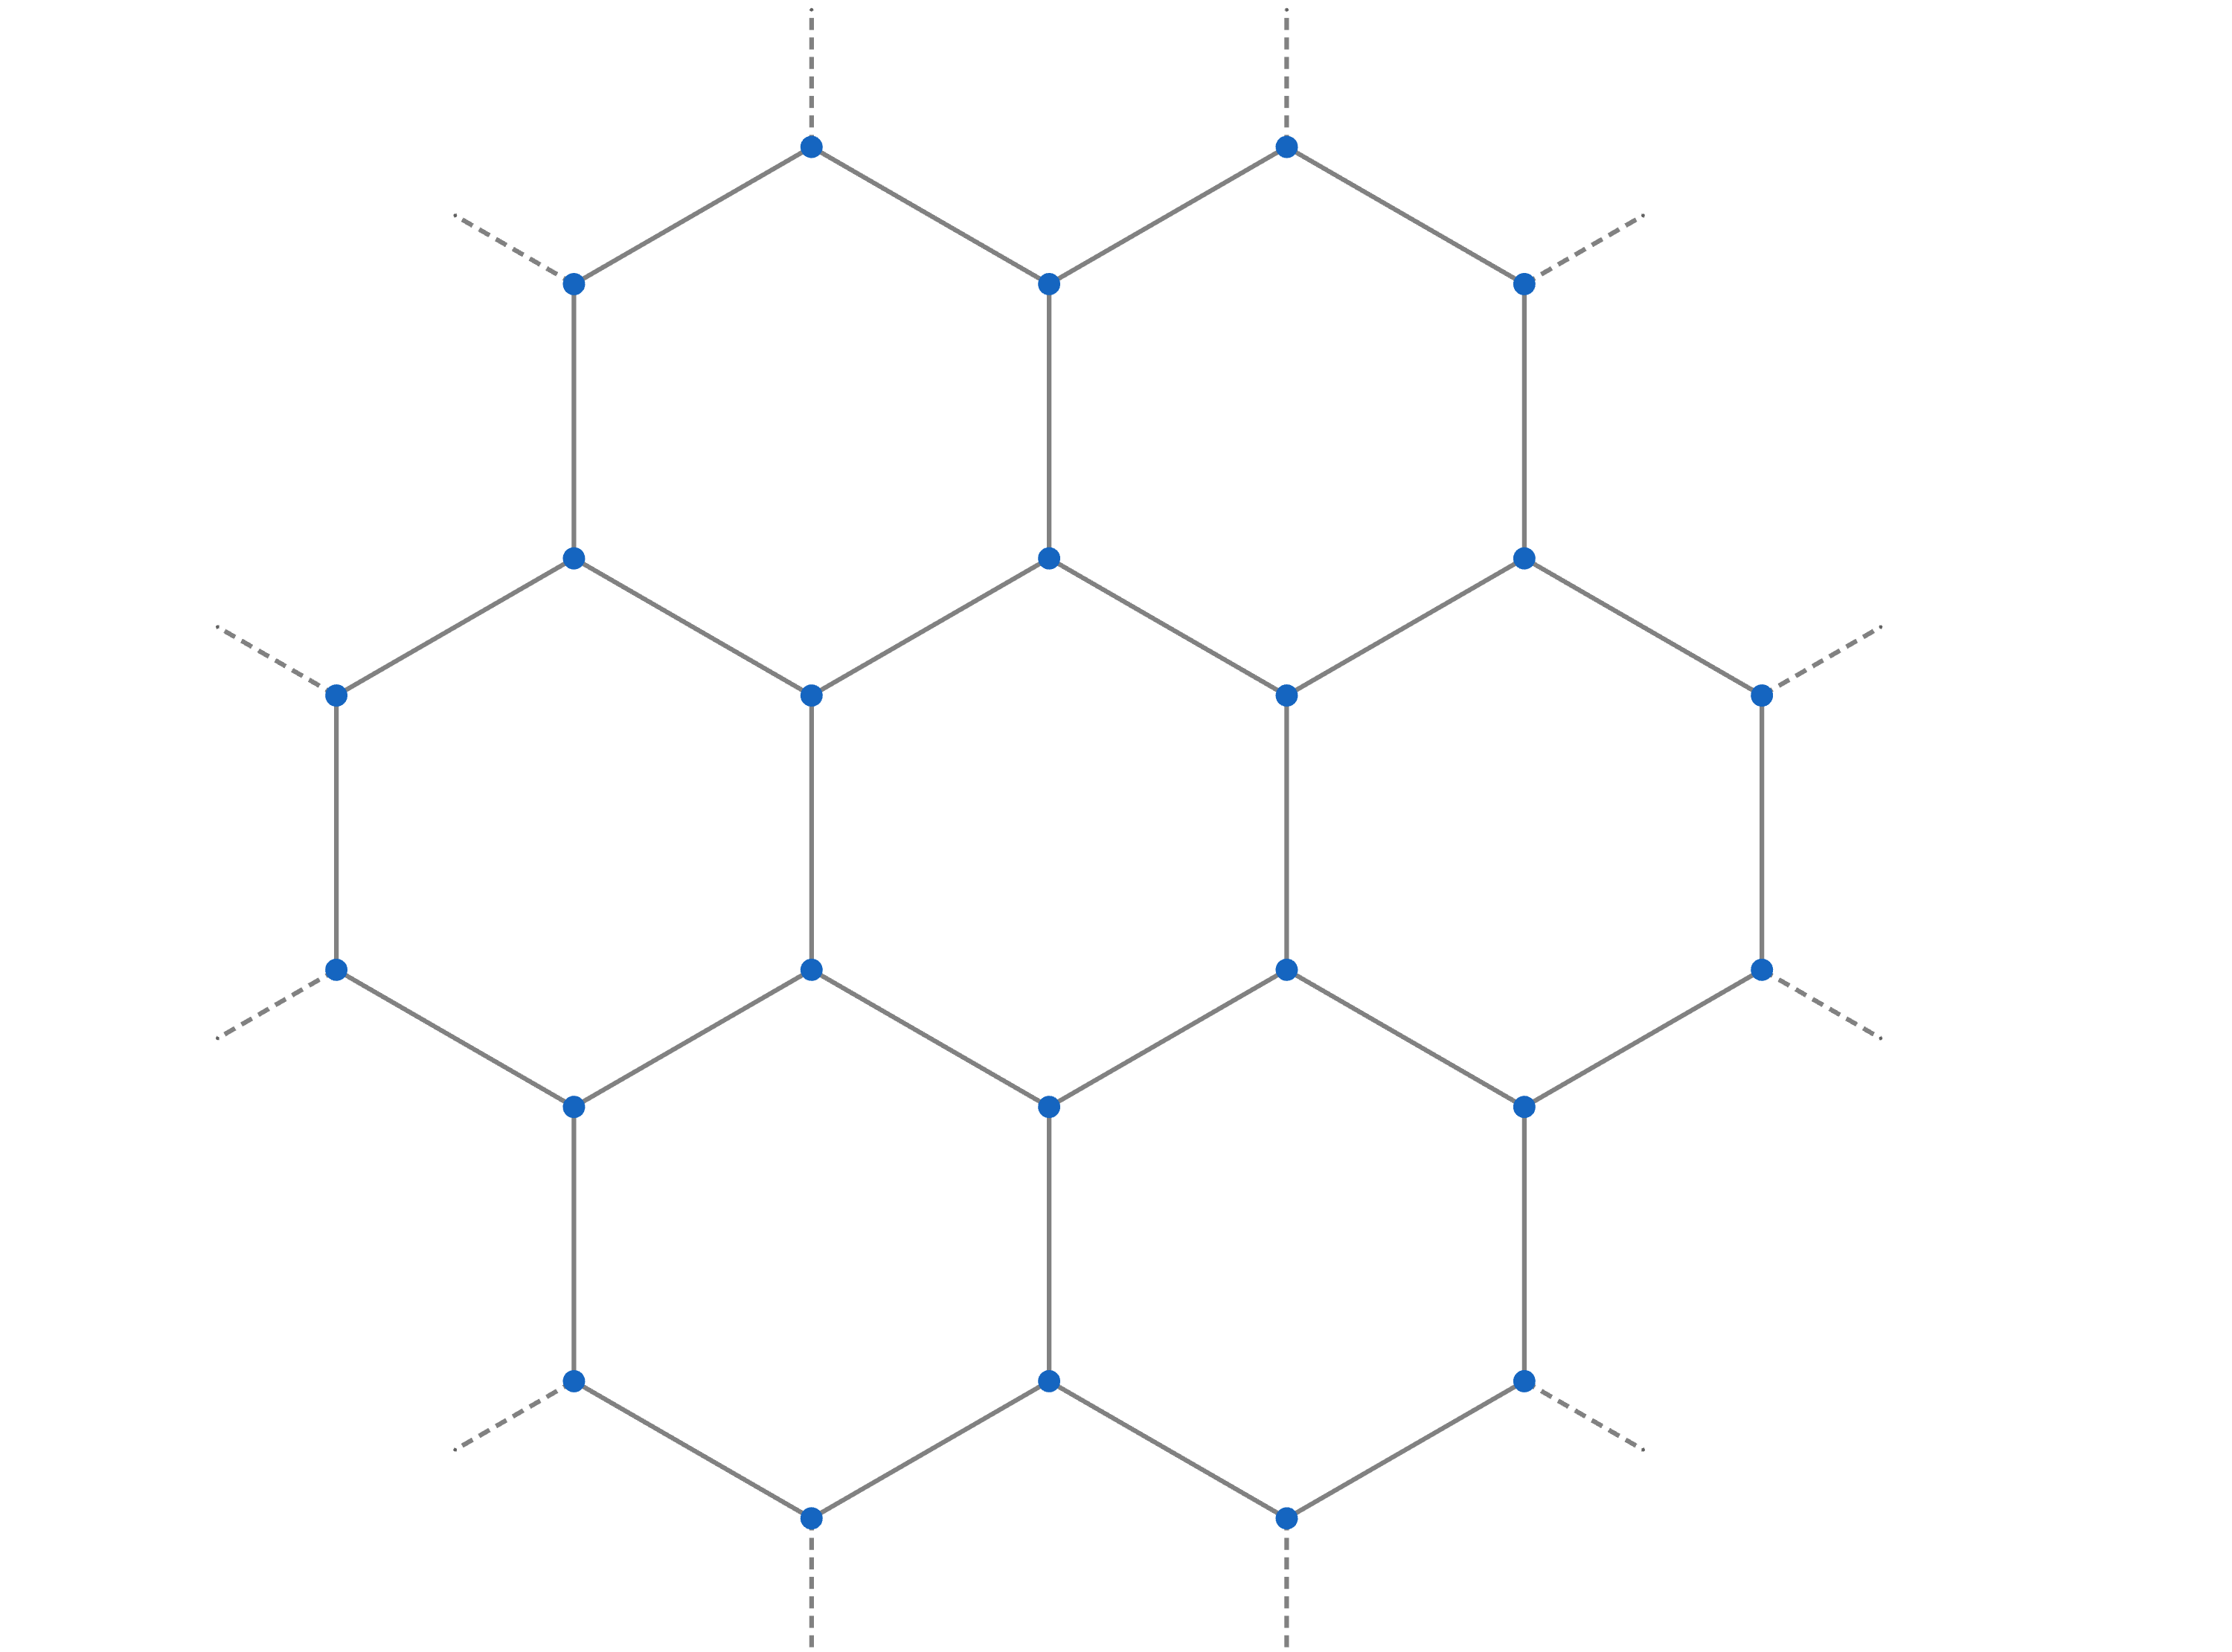
\includegraphics[width=4cm]{gfx/triangle group cayley graph.png}}}%\newline
    \subfloat[\centering \(D_\infty\)]{{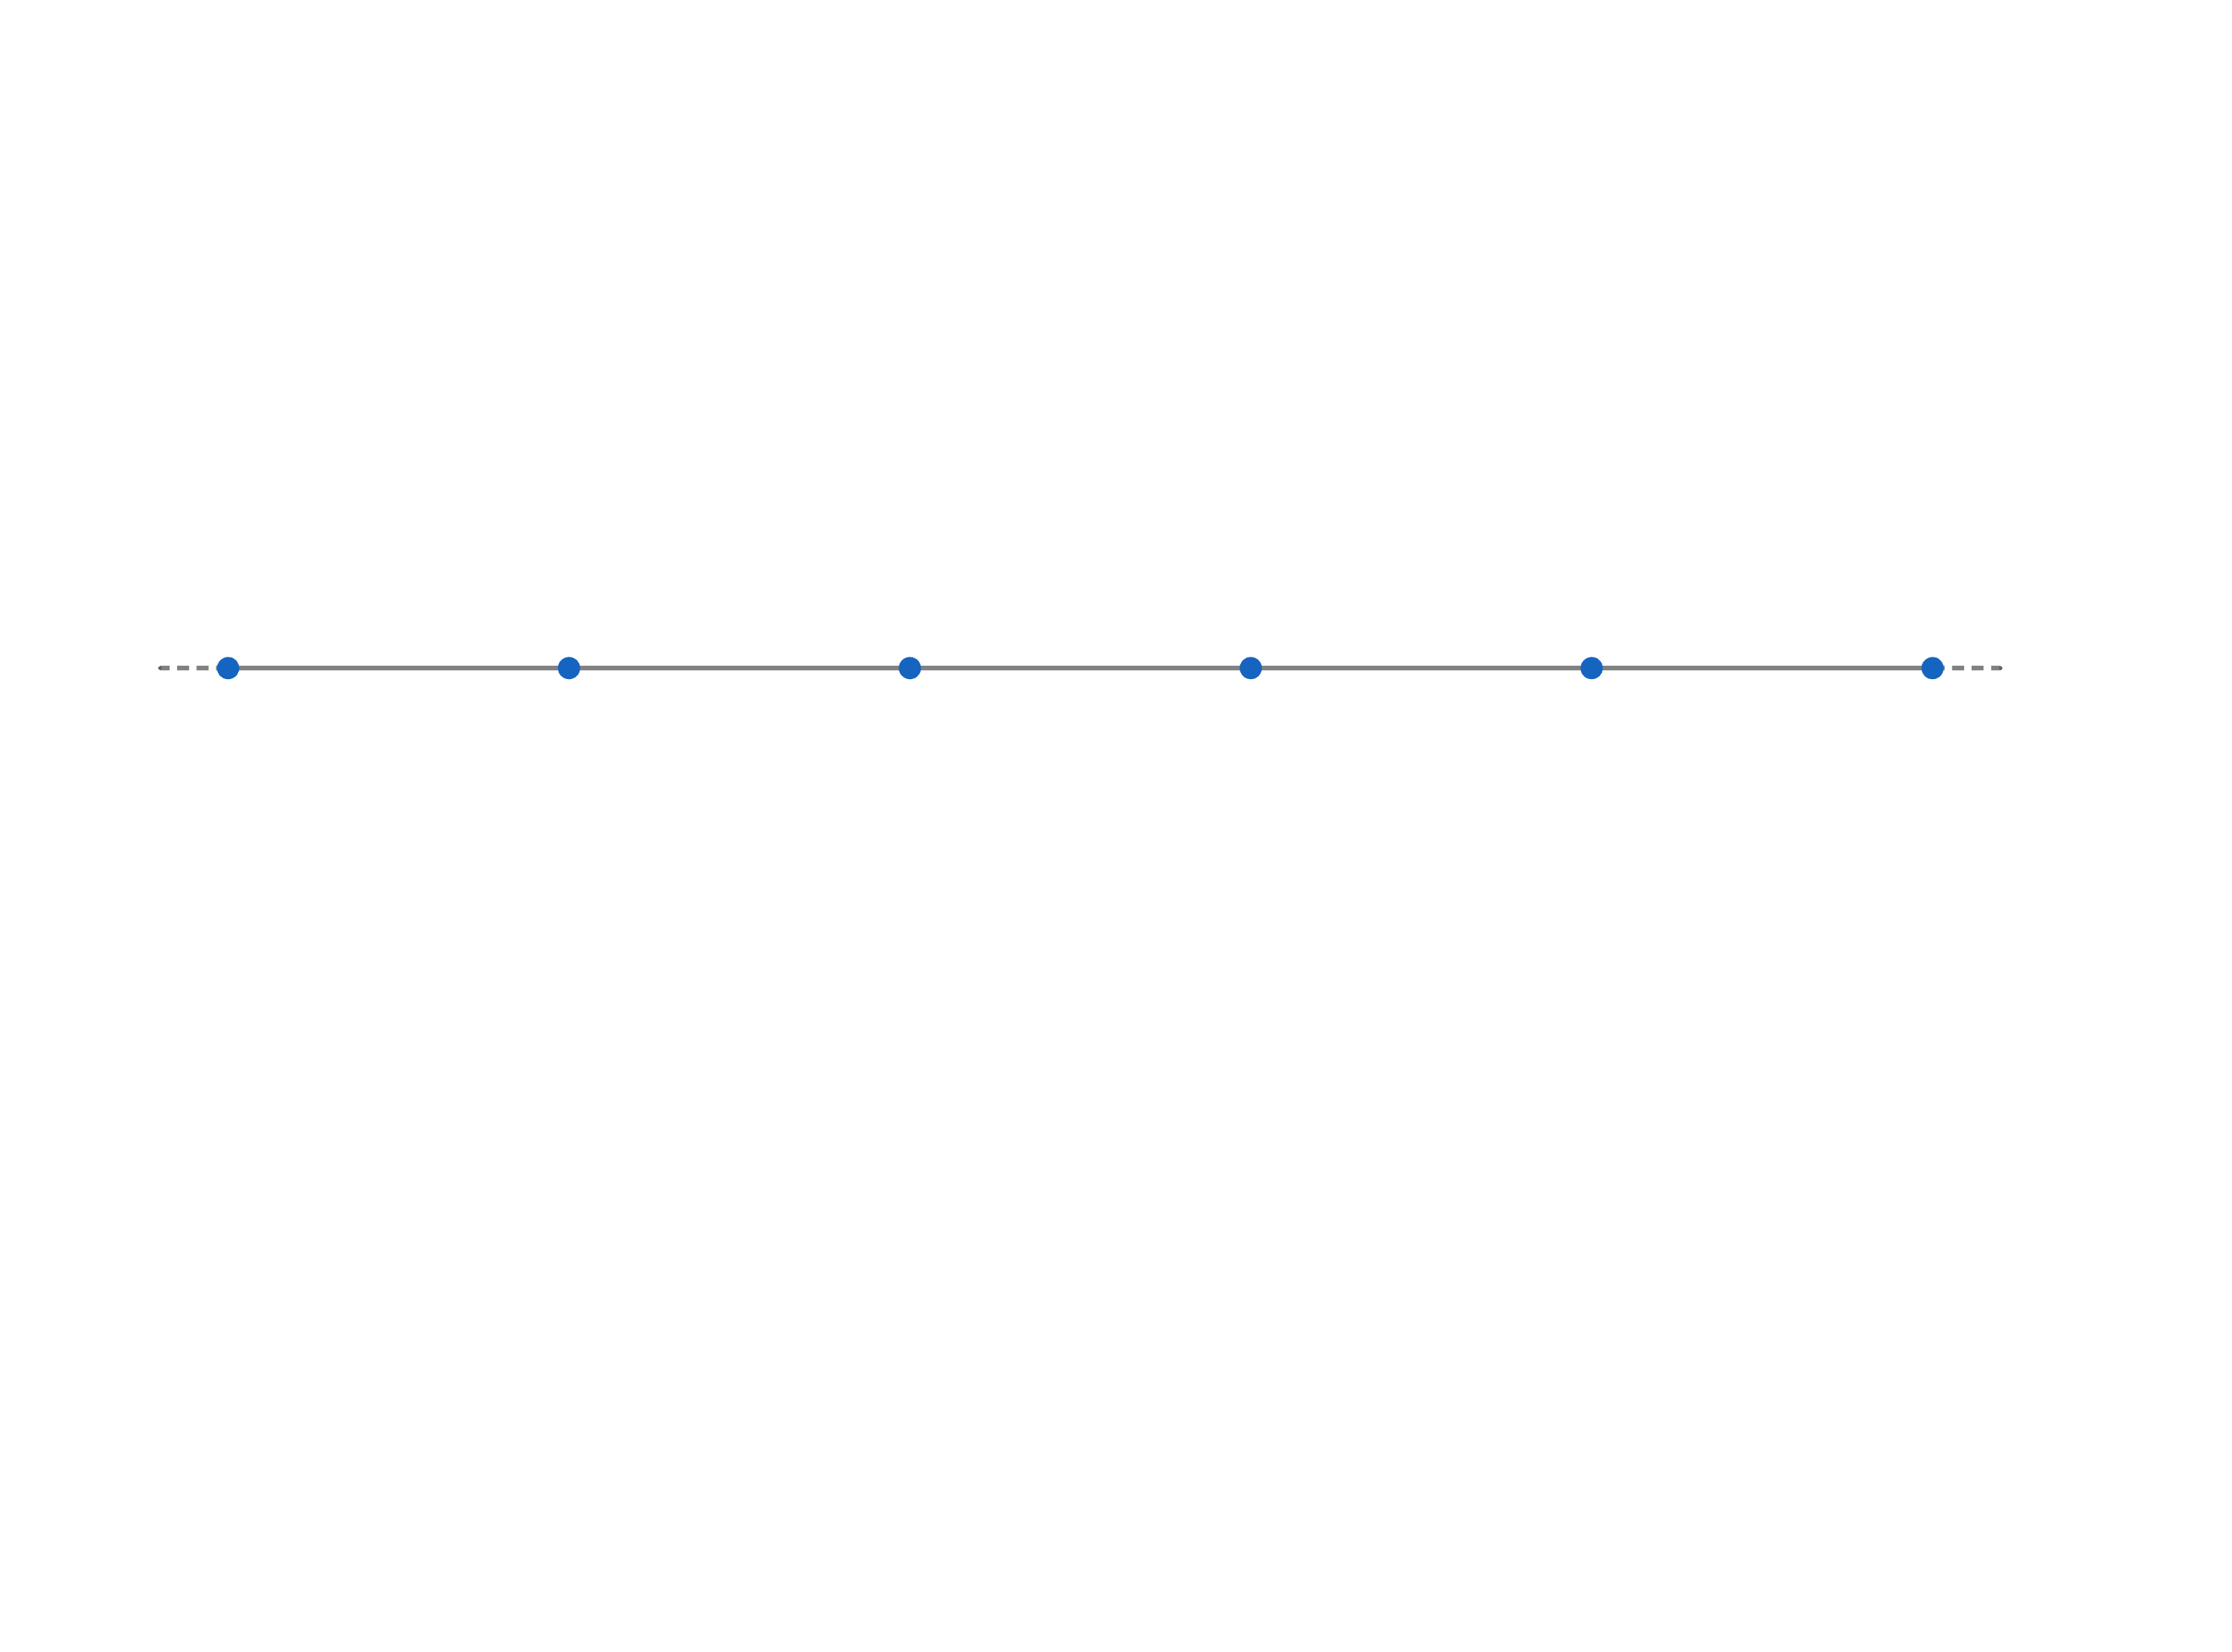
\includegraphics[width=4cm]{gfx/infinite dihedral cayley graph.png}}}
    \subfloat[\centering \(\faktor{\Z}{2\Z}\ast\faktor{\Z}{2\Z}\ast\faktor{\Z}{2\Z}\)]{{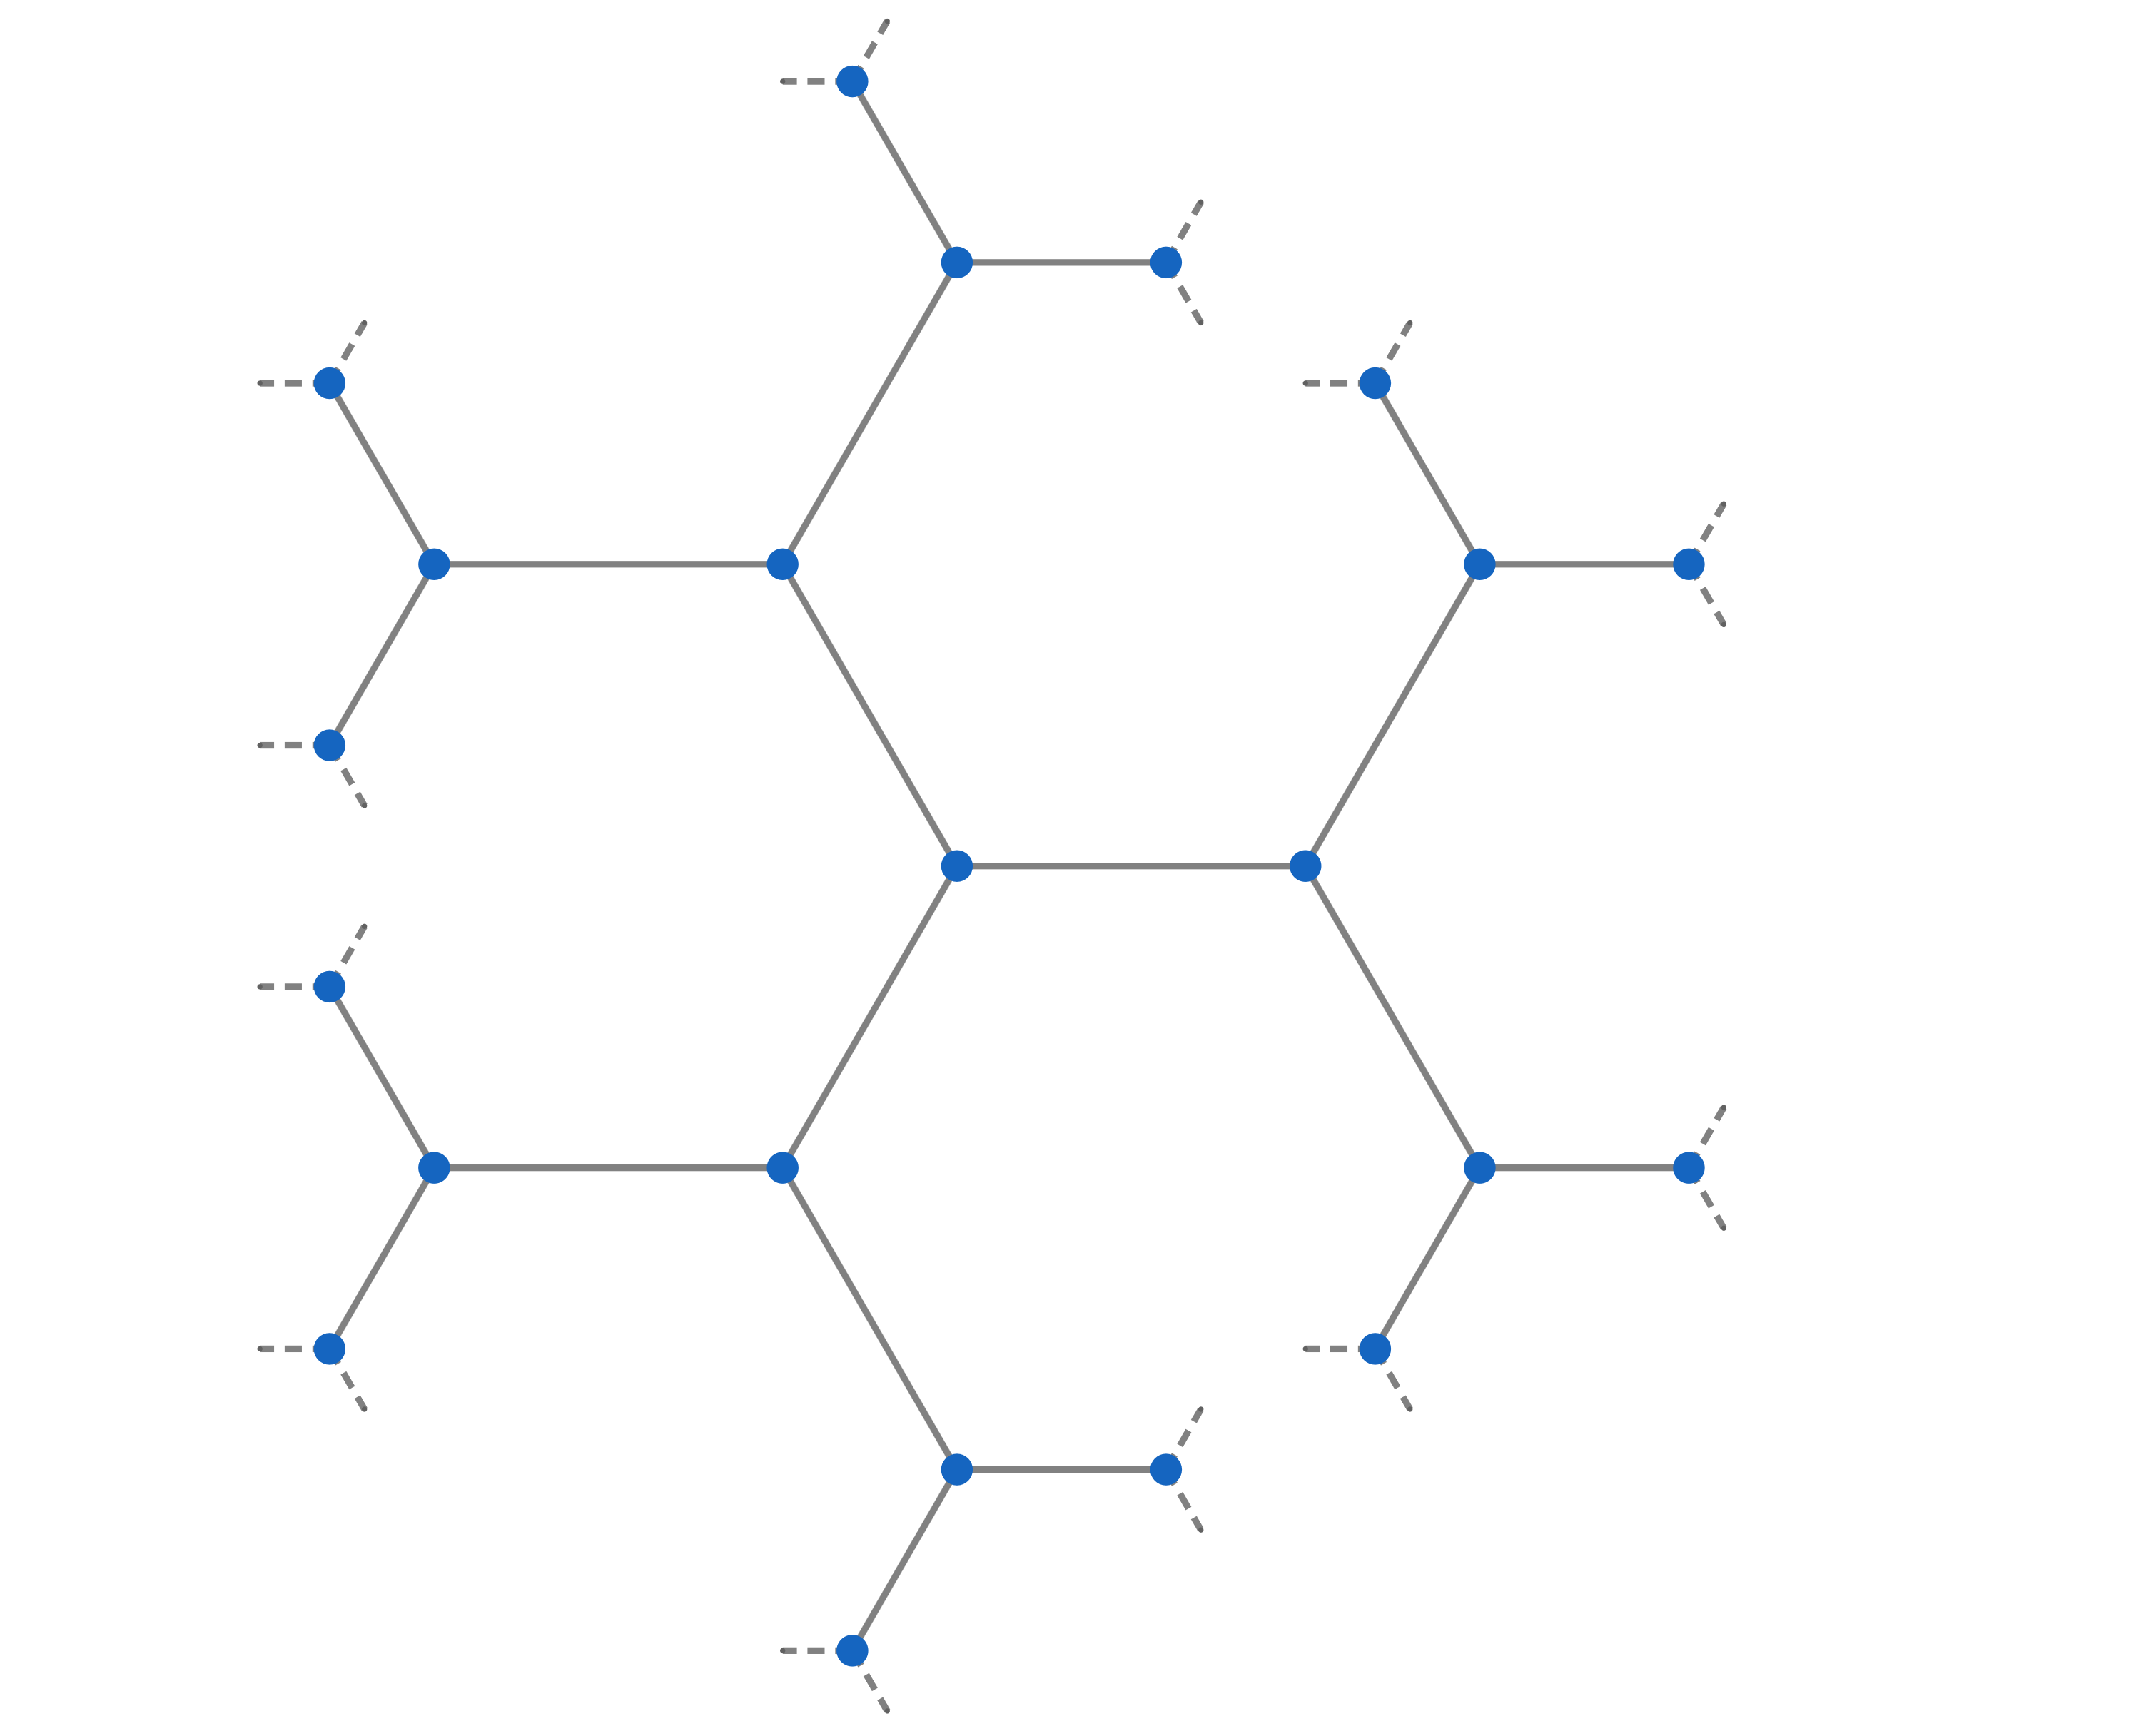
\includegraphics[width=4cm]{gfx/free product cayley graph.png}}}
\end{figure}

We define a special type of subgroups, called parabolic subgroups within a Coxeter group \(W\).
These subgroups are constructed from a subset of the index set \(I\).
The definition is as follows:

\begin{definition}
    Let \((W,S)\) be a Coxeter System as above with finite index set \(I\), and \(J\) be a subset of the index set \(I\).
    The group \(W_J := \langle\{s_j \;\vert\; j\in J\}\rangle\), generated by the \(s_j\) in \(S\) with \(j \in J\), is then called a \emph{parabolic subgroup} of \(W\).
    Moreover, we call any conjugate of \(W_J\) a parabolic subgroup as well.
\end{definition}

Once we have constructed the representation of Coxeter groups on a vector space as well as the Tits cone in the coming section, the parabolic subgroups will be a useful tool to form a deeper understanding of these objects.
We will extensively use them in Sections \(2.4\) and \(2.5\).

% ***********************************************
\section{Representation of Coxeter groups}
% ***********************************************

Given a Coxeter System \((W,S)\), let \(V\) be a real vector space with basis \(\{e_1,\ldots,e_n\}\), where \(n=\abs{I}=\abs{S}\).
This provides a natural identification, \(GL_n(V)\cong GL_n(\R)\).
We define a bilinear form \(B_W\) on \(V\) as follows:
\begin{equation*}
    B_W(e_i, e_j) := \begin{cases}
        -\cos \left(\frac{\pi}{m_{ij}}\right) & ,\; m_{ij}<\infty \\
        -1                                    & ,\; m_{ij}=\infty
    \end{cases}.
\end{equation*}
By \Cref{def:CoxeterGroup}, it is assured that \(m_{ij}\geq 2\) for distinct \(i,j\), ensuring the cosine term is non-positive.
Consequently, we have \(B_W(e_i,e_j)\leq 0\) for distinct \(i,j\).
Furthermore, from \(m_{ii}=1\), it follows that \(B_W(e_i,e_i)=1\).
Using this bilinear form, we define hyperplanes with corresponding reflections for each basis element \(e_i\) as follows:
\[H_i := \{v\in V\;\vert\; B_W(e_i,v) = 0\}\;, \qquad \sigma_i : V\to V,\quad v\mapsto v - 2B_W(e_i,v)e_i.\]

\begin{theorem}\label{thm:repr}
    The map given by:
    \[\rho : W \to GL_n(V) \cong GL_n(\R), \quad s_i \mapsto \sigma_i\]
    is an injective homomorphism and therefore a faithful representation of \(W\).
\end{theorem}
Before we prove the homomorphism property, we recall:
A map \(\varphi: S\to G\) from a set \(S\) to a group \(G\) extends to a homomorphism \(\Hat{\varphi}:\groupp{S}{R}\to G\), if and only if the induced homomorphism \(\overline{\varphi}:F_S \to G\) from the free group over \(S\) satisfies \(\overline{\varphi}(r) = 1_G\) for every \(r\in R\).
\begin{proof}
    Observe that \(\sigma_i^2 = id\) in \(GL_n(V)\) and thus to prove that \(\rho\) is a homomorphism, we apply the above to our situation to see that it suffices to show that the product \(\sigma_i\sigma_j\) has order \(m_{ij}\) in \(GL_n(V)\) for distinct \(i,j\in I\).
    Also note that in the case of \(m_{ij} = \infty\) there is nothing to prove as these relations are defined to be trivial in the presentation of \(W\).
    
    Thus, consider the two-dimensional subspace \(V_{ij}\) of \(V\) spanned by two basis vectors \(e_i, e_j\) and take a general element \(v = \lambda \cdot e_i + \mu \cdot e_j\) in \(V_{ij}\) with \(\lambda, \mu \in \R\) not simultaneously zero.
    As \(m_{ij} < \infty\), the bilinear form \(B_W\) is positive definite by the following calculation
    \[B_W (v,v) = \lambda^2 - 2\lambda\mu\cos\left(\frac{\pi}{m_{ij}}\right) + \mu^2 = \left(\lambda - \mu \cos\left(\frac{\pi}{m_{ij}}\right)\right)^2 + \mu^2\sin^2\left(\frac{\pi}{m_{ij}}\right) > 0.\]
    Identify \((V_{ij}, B_W\vert_{V_{ij}})\) with the euclidean plane \((\R^2, \langle \cdot, \cdot \rangle)\) up to a change of basis.
    Then \(\sigma_i\), resp. \(\sigma_j\) act by orthogonal reflections in their corresponding hyperplanes \(H_i\), resp. \(H_j\) intersected with \(V_{ij}\).
    By having a look at the inner product of \(e_i\) and \(e_j\)
    \[B_W(e_i, e_j) = - \cos\left(\frac{\pi}{m_{ij}}\right) = \cos\left(\pi - \frac{\pi}{m_{ij}}\right),\]
    we observe that the angle between the two in \(V_{ij}\) is precisely \(\pi - \frac{\pi}{m_{ij}}\).
    We conclude from this that the angle between their reflecting lines in \(\frac{\pi}{m_{ij}}\) and the composition \(\sigma_i\sigma_j\) turns out to be a rotation about \(\frac{2\pi}{m_{ij}}\).
    As the composition \(\sigma_i\sigma_j\) fixes the orthogonal complement \(V_{ij}^\perp\) of \(V_{ij}\) by definition of the \(\sigma_i\), we see that it has order \(m_{ij}\) on the whole space \(V\).
    % To do so, consider the two-dimensional subspace \(V_{ij}\) spanned by two basis vectors \(e_i\) and \(e_j\) in \(V\).
    % We take a general element \(v = \lambda e_i + \mu e_j\), \(\lambda,\mu\in\R\) in \(V_{ij}\) and distinguish the two cases in the definition of \(B_W\):
    % \begin{itemize}
    %     \item[1)] \(m_{ij}<\infty\): In this case \(B_W\) is positive definite, since for \(v\neq 0\)
    %           \begin{align*}
    %               B_W(v,v) & = \lambda^2 - 2\lambda\mu\cos\left(\frac{\pi}{m_{ij}}\right) + \mu^2
    %               = \left( \lambda - \mu\cos\left( \frac{\pi}{m_{ij}} \right) \right)^2 + \mu^2\sin^2\left( \frac{\pi}{m_{ij}} \right) > 0.
    %           \end{align*}
    %           Up to a change of basis, we identify \((V_{ij}, B_W\vert_{V_{ij}})\) with the euclidean plane \((\R^2, \langle\cdot, \cdot\rangle)\).
    %           Now \(\sigma_i\) and \(\sigma_j\) act on \(V_{ij}\) by orthogonal reflections in the hyperplanes \(H_i, H_j\) intersected with \(V_{ij}\).
    %           We take a look at the inner product of \(e_i, e_j\)
    %           \[B_W(e_i, e_j) = -\cos\left(\frac{\pi}{m_{ij}}\right) = \cos\left(\pi - \frac{\pi}{m_{ij}}\right)\]
    %           and obtain that the angle between them in \(V_{ij}\) is given by \(\pi - \frac{\pi}{m_{ij}}\).
    %           Thus, the angle between the reflecting lines is \(\frac{\pi}{m_{ij}}\) and the product \(\sigma_i\sigma_j\) turns out to be a rotation by \(\frac{2\pi}{m_{ij}}\), showing that \(\sigma_i\sigma_j\) has order \(m_{ij}\) in the subspace \(V_{ij}\).
    %           And since \(\sigma_i\sigma_j\) fixes the orthogonal complement of \(V_{ij}\) by definition of the \(\sigma_i\), it has order \(m_{ij}\) on the whole vector space \(V\).

    %     \item[2)] \(m_{ij} = \infty:\;\) By the following, we now have to deal with a non-positive definite form:
    %           \begin{align*}
    %               B_W(v,v) = \lambda^2 - 2\lambda\mu + \mu^2 = (\lambda - \mu)^2 \geq 0.
    %           \end{align*}
    %           Indeed, we can only expect it to be positive semidefinite on \(V_{ij}\).
    %           Using the calculation
    %           \begin{align*}
    %               (\sigma_i\sigma_j)(e_i) = \sigma_i (e_i + 2e_j) = e_i + 2(e_i + e_j),
    %           \end{align*}
    %           together with an induction argument, we get that \((\sigma_i\sigma_j)^n(e_i) = e_i + 2n(e_i + e_j)\).
    %           Therefore, the concatenation has infinite order on \(V_{ij}\) and in particular on the whole of \(V\).
    % \end{itemize}
    This proves that \(\rho\) extends to a homomorphism.
    It remains to show the injectivity of \(\rho\).
    This will be a consequence of a bigger result in section \(2.4\), see \Cref{cor:faithful}.
\end{proof}

In contrast to the above proof, in the case of \(m_{ij} = \infty\), we cannot expect our bilinear form to be positive definite.
Let \(v \in V_{ij}\) be as in the proof, then
\[B_W(v,v) = \lambda^2 - 2\lambda\mu + \mu^2 = (\lambda - \mu)^2 \geq 0.\]
This shows that we can at least expect it to be positive semidefinite.
The direct calculation
\[(\sigma_i\sigma_j)(e_i) = \sigma_i(e_i + 2e_j) = e_i + 2(e_i + e_j),\]
together with an inductive argument, shows that \((\sigma_i\sigma_j)^n(e_i) = e_i + 2n(e_i + e_j)\).
Therefore, the composition \(\sigma_i\sigma_j\) has infinite order on \(V_{ij}\) and in particular on the whole of \(V\).
The following remark is a consequence of this, together with the observation in above proof.

\begin{remark}
    From last paragraph and the proof of \Cref{thm:repr}, we conclude that two-generator subgroups of Coxeter groups are dihedral.
    Either of order \(2m_{ij}\) or infinite order.
\end{remark}

We want to extend the action of \(W\) to the dual of the vector space \(V\).
This is achieved by acting on \(V^*\) via the dual representation of \(\rho\), which we define by
\[\rho^* : W \to GL_n(V^*),\quad w \mapsto (\rho^*(w): V^* \to V^*, \; \varphi \mapsto \rho^*(w)(\varphi)), \quad w\in W, \varphi\in V^*.\]
We can evaluate the functional \(\rho^*(w)(\varphi)\) on some \(v \in V\) via \((\rho^*(w)(\varphi))(v) := \varphi(\rho(w^{-1})(v))\).
Notation wise, we will simply write \(w(v)\), when \(w \in W\) acts on \(v \in V\) via \(\rho(w)(v)\).
Similarly, we write \(w(\varphi)\) when we mean that \(w \in W\) acts on some element \(\varphi \in V^*\) of the dual space, via the dual representation \(\rho^*(w)(\varphi)\).
As in the case of the vector space \(V\), we want to give a definition for the notion of a hyperplane with corresponding reflection in the dual space \(V^*\) as well.
By dual hyperplane, we mean a subspace \(H_i^* := \{\varphi \in V^* \;\vert\; \varphi (e_i) = 0\}\), and the corresponding dual reflections will be a map from \(V^*\) to \(V^*\), given by:
\[\sigma_i^* : V^* \to V^*,\quad \varphi \mapsto \varphi \circ \sigma_i = \varphi - 2B_W(e_i,\;\cdot\;)\varphi(e_i).\]

To further explore Coxeter groups and their action via this representation, we need some more notation.
In particular, we want a so-called \emph{chamber}.
This should be thought of as a cone over a polytope with finitely many faces such that the reflections in its codimension one faces correspond to the generators of \(W\) under the representation.

\begin{definition}\label{def:chamber}
    The fundamental chamber \(C\) of the dual representation is the set, given by
    \[C := \{\varphi \in V^* \;\vert\; \varphi (e_i) \geq 0 \;\forall i\in I\} \subset V^*.\]
\end{definition}

Denote by \(\{e_1^*,\ldots, e_n^*\}\) the dual basis of \(V^*\) corresponding to the standard basis \(\{e_1,\ldots, e_n\}\) of \(V\).
Then we calculate, using the \(\sigma_i^*\) from above:
\begin{equation*}
    \sigma_i^*(e_j^*) = e_j^* - 2B_W(e_i,\cdot)e_j^*(e_i) =
    \begin{cases}
        e_j^*                   & \text{for } i\neq j \\
        e_j^* - 2B_W(e_j,\cdot) & \text{for } i=j
    \end{cases},
\end{equation*}
which implies that each reflection \(\sigma_i^*\) fixes all the hyperplanes \(H_j^*\), for distinct indices \(i\) and \(j\).
Moreover, note that the fundamental chamber can be written in the form % TODO: rework the following paragraph --
\[C = \bigcap_{i\in I}\{\varphi\in V^*\;\vert\; \varphi(e_i)\geq 0\} = \bigcap_{i\in I} (H_i^* \cup \{\varphi\in V^*\;\vert\; \varphi(e_i)> 0\}),\]
where we observe that the sets \(H_i^*\cap C\) form the pairwise distinct codimension one faces of the chamber \(C\).
The open halfspaces \(\{\varphi \in V^* \;\vert\; \varphi(e_i) > 0\}\) in the latter term will be called \(A_i^*\) and using these, we define the open fundamental chamber to be the intersection of the open halfspaces:
\[\text{int}(C) = \mathring{C} = \bigcap_{i \in I} A_i^*.\] % ---------
As mentioned above, we want to study the action of our Coxeter group via the dual representation, acting by reflection in the faces \(H_i^*\).
However, in general the translates of the chamber under the group action won't cover the whole of \(V^*\), which motivates the following definition:

\begin{definition}
    The Tits cone is the union of all \(W\)-translates of the chamber, \(WC := \underset{w \in W}{\bigcup} wC \subset V^*\).
\end{definition}

As the name suggests, the fundamental chamber is a fundamental domain for the action of \(W\) on its Tits cone \(WC\) under the dual representation \(\rho^*\).
This will be proved in \Cref{thm:funddomain}.
While the formal defintion of the Tits cone provides a rigorous foundation, it is not very insightful from a geometric perspective.
As one can think about the Tits cone quite geometrically, especially in low dimensions, we will take a closer look at an explicit example in the following section.
Before doing so, we end this section with the following remark.

\begin{remark} % TODO: add picture
    One may ask why we transport everything to the dual space, instead of working in the standard representation \(\rho\).
    For this, consider the infinite dihedral group \(D_\infty \cong \groupp{s, t}{s^2 = t^2 = 1}\).
    We fix a basis \(\{e_1, e_2\}\) of \(V\) and obtain that the bilinear form in this basis is given by the matrix
    \begin{equation*}
        B_W = \begin{pmatrix}
            1  & -1 \\
            -1 & 1
        \end{pmatrix}.
    \end{equation*}
    We observe that \(H_1 = \text{span}\{e_1 + e_2\} = H_2\), which implies that \(\sigma_1\) and \(\sigma_2\) fix the same hyperplane, despite having different \((-1)\)-Eigenspaces (namely the span of \(e_1\), resp. \(e_2\)).
    Therefore, in general, working in the standard representation won't result in a chamber, giving rise to the existence of the Tits cone.
    Now, passing to the dual space \(V^*\) by fixing the dual basis \(\{e_1^*, e_2^*\}\), consider the dual reflections \(\sigma_i^*\) as discussed before.
    By the more general calculation earlier, we obtain
    \[\sigma_1^*(H_2^*) = H_2^* \quad\text{and}\quad \sigma_2^*(H_1^*) = H_1^*.\]
    And furthermore, we note that for all \(i,j\in\{1,2\}\)
    \[\sigma_i^*(B_W(e_j,\cdot)) = B_W(e_j,\cdot) - 2B_W(e_i,\cdot)B_W(e_j,e_i) = - B_W(e_j,\cdot),\]
    using that \(B_W(e_j,\cdot) = -B_W(e_i,\cdot)\).
    This shows that both dual reflections have the same \((-1)\)-Eigenspace, but fix different hyperplanes (\ie, have different \((+1)\)-Eigenspaces), resulting in a chamber as wished.
\end{remark}


% ***********************************************
\section{The Tits cone - An example} % TODO: add picture
% ***********************************************

As an example we take a closer look at the free product \(W \cong\groupp{r,s,t}{r^2=s^2=t^2=1}\), a right-angled Coxeter group from \Cref{ex:freeprod}.
We fix the basis \(\{e_1,e_2,e_3\}\) and identify \(V\) with \(\R^3\).
In this basis, the bilinear form \(B_W\) is given by the matrix
\begin{equation*}
    B_W =
    \begin{pmatrix}
        1  & -1 & -1 \\
        -1 & 1  & -1 \\
        -1 & -1 & 1
    \end{pmatrix}.
\end{equation*}
By the spectral theorem we find a basis of orthonormal Eigenvectors, in which \(B_W\) is a diagonal matrix with its eigenvalues as entries.
Using the Gram-Schmidt procedure, we get
\begin{equation*}
    \begin{pmatrix}
        -\frac{1}{\sqrt{2}} & 0                  & \frac{1}{\sqrt{2}}  \\
        -\frac{1}{\sqrt{6}} & \frac{2}{\sqrt{6}} & -\frac{1}{\sqrt{6}} \\
        \frac{1}{\sqrt{3}}  & \frac{1}{\sqrt{3}} & \frac{1}{\sqrt{3}}
    \end{pmatrix} \cdot
    \begin{pmatrix}
        1  & -1 & -1 \\
        -1 & 1  & -1 \\
        -1 & -1 & 1
    \end{pmatrix} \cdot
    \begin{pmatrix}
        -\frac{1}{\sqrt{2}} & -\frac{1}{\sqrt{6}} & \frac{1}{\sqrt{3}} \\
        0                   & \frac{2}{\sqrt{6}}  & \frac{1}{\sqrt{3}} \\
        \frac{1}{\sqrt{2}}  & -\frac{1}{\sqrt{6}} & \frac{1}{\sqrt{3}}
    \end{pmatrix} =
    \begin{pmatrix}
        2 & 0 & 0  \\
        0 & 2 & 0  \\
        0 & 0 & -1
    \end{pmatrix}.
\end{equation*}
In other words, we have \(V^T B_W V = D\) with \(V\in O(n)\) and \(D = \text{diag}(2,2,-1)\).
Now, since we have a diagonal matrix, we can multiply the entries by squares, since the resulting matrix will be congruent to the given one:

Let \(A = \text{diag}(\mu_1,\ldots,\mu_n)\in\R^{n\times n}\),
\begin{equation*}
    S=\text{diag}(\lambda_1,\ldots, \lambda_n)\in(\R\setminus\{0\})^{n\times n} \implies S^TAS = \text{diag}(\lambda_1^2\mu_1,\ldots,\lambda_n^2\mu_n).
\end{equation*}
To apply this and further transform our matrix \(D\), define the invertible matrix \(T\) as follows
\[T = \begin{pmatrix} \frac{1}{\sqrt{2}} & 0 & 0 \\ 0 & \frac{1}{\sqrt{2}} & 0 \\ 0 & 0 & 1 \end{pmatrix},\]
which then implies \(\widetilde{D} := T(V^T B_W V)T = \text{diag}(1,1,-1)\).
The images of the basis vectors \(\{e_1,e_2,e_3\}\) are given by the three columns of the matrix \(TV^T\), namely:
\begin{equation*}
    \widetilde{e}_1 = \begin{pmatrix} -\frac{1}{2} \\ - \frac{\sqrt{3}}{6} \\ \frac{1}{\sqrt{3}} \end{pmatrix},\;
    \widetilde{e}_2 = \begin{pmatrix} 0 \\ \frac{1}{\sqrt{3}} \\ \frac{1}{\sqrt{3}} \end{pmatrix} \text{ and }
    \widetilde{e}_3 = \begin{pmatrix} \frac{1}{2} \\ -\frac{\sqrt{3}}{6} \\ \frac{1}{\sqrt{3}} \end{pmatrix}.
\end{equation*}
Note that we have \(V\cong \R^3\), equipped with the inner product
\[\langle x, y \rangle_{2,1} := x^T\widetilde{D}y = x_1y_1 + x_2y_2 - x_3y_3.\]
Since \(\langle \widetilde{e}_i, \widetilde{e}_i \rangle_{2,1} = 0\) for all \(i\in \{1,2,3\}\), we have that these three vectors span an ideal triangle in the hyperboloid model of \(\HH^2\), given by \(\langle x, y \rangle_{2,1} = -1\).
One gets the ideal triangle by intersecting the hyperboloid with the hyperplanes spanned by each two of the \(\widetilde{e}_i\) (they will only intersect in the surrounding cone of the hyperboloid).

Given these new coordinates under the transformation \(TV^T\), the Tits cone will be given by \(x_1^2 + x_2^2 - x_3^2 < 0\) union the images of \(\widetilde{e}_1, \widetilde{e}_2\) and \(\widetilde{e}_3\) under the reflection in the sides of the chamber, i.e. in the sides of the ideal triangle. % TODO: under the transformation TV^t
Moreover, we get a subgroup of \(O(2,1)_+\) generated by the following three matrices
\begin{equation*}
    \begin{pmatrix} 1 & 0 & 0 \\ 0 & -\frac{5}{3} & -\frac{4}{3} \\ 0 & \frac{4}{3} & \frac{5}{3} \end{pmatrix},\;
    \begin{pmatrix} -1 & \frac{2}{\sqrt{3}} & -\frac{2}{\sqrt{3}} \\ \frac{2}{\sqrt{3}} & \frac{1}{3} & \frac{2}{3} \\ \frac{2}{\sqrt{3}} & -\frac{2}{3} & \frac{5}{3} \end{pmatrix}
    \text{ and }
    \begin{pmatrix} -1 & -\frac{2}{\sqrt{3}} & \frac{2}{\sqrt{3}} \\ -\frac{2}{\sqrt{3}} & \frac{1}{3} & \frac{2}{3} \\ -\frac{2}{\sqrt{3}} & -\frac{2}{3} & \frac{5}{3} \end{pmatrix}.
\end{equation*}
Each of the above matrices corresponds to one of the generators \(r, s\) and \(t\) of the right angled Coxeter group \(W\) under the transformation \(TV^T\), constructed above.


% ***********************************************
\section{The word metric and the faithful representation}
% ***********************************************

Recall that for any finitely generated group \(W = \langle S \rangle\), its Cayley graph induces a metric on \(W\), relative to the generating set \(S\).
We call it the \emph{word metric} of \(W\) relative to \(S\) and denote it by \(d_S\).
Also note that the word metric is left-invariant, meaning that for group elements \(u,v,w\in W\), we have the equality \(d_S(uv,uw) = d_S(v,w)\).
Now, define the \emph{word length} of an element \(w\in W\) to be \(\ell(w) := d_S(w, 1_W)\), the distance of an element to the neutral element of the group.
Note that \(\ell(w) = 0\) if and only if \(w = 1_W\).

\begin{lemma}
    We collect some properties of the length function we will use later on.
    \begin{enumerate}
        \item \(\forall w\in W:\; \ell(w) = \ell(w^{-1})\)
        \item \(\forall s\in S:\; \ell(s) = 1\) and \(\ell(w) = 1 \iff w\in S^{\pm 1}\)
        \item \(\forall v,w\in W:\; \ell(vw)\leq\ell(v)+\ell(w)\)
        \item \(\forall v,w\in W:\; \ell(v)-\ell(w)\leq\ell(vw)\)
        \item \(\forall w\in W, s\in S^{\pm 1}:\; \ell(w)-1\leq\ell(ws)\leq\ell(w)+1\)
    \end{enumerate}
\end{lemma}
\begin{proof}
    All of the above statements follow from the fact that \(d_S\) is a left-invariant metric.
    % \begin{enumerate}
    %     \item For \(w\in W\), write the length of w as \(\ell(w) = d_S(w, e_W)\).
    %           By the left-invariance of \(d_S\), we have \(d_S(w, e_W) = d_S(e_W, w^{-1})\) and by symmetry of \(d_S\), \(\ell(w) = \ell(w^{-1})\) follows.
    %     \item This is true by definition.
    %     \item For \(u,v\in W\), using the triangle inequality of \(d_S\), we get: \[\ell(uv) = d_S(uv, e_W) \leq d_S(u, e_W) + d_S(v, e_W) = \ell(u) + \ell(w).\]
    %     \item For \(v,w\in W\) we have \(\ell(v)=\ell(vww^{-1})\leq\ell(vw) + \ell(w^{-1})\), by point 3 and thus, using point 1: \(\ell(v) - \ell(w) \leq \ell(vw)\).
    %     \item For \(w\in W,\; s\in S\), apply point 3 and point 4 to \(\ell(ws)\).
    % \end{enumerate}
\end{proof}

Coming back to Coxeter groups, by definition each generator \(s\in S\) has order 2 in \(W\).
Therefore, we can write every non-trivial element in \(W\) as a sequence of generators in \(S\).
Note that in this sequence there might be redundencies, so that the following definition makes sense.
We call an expression \(w = s_{i_1} \cdots s_{i_r}\) for \(i_1,\ldots, i_r\in I\) and \(r\in\N\) \emph{reduced}, if \(\ell(w) = r\), \ie \(\;w\) cannot be represented by a shorter word.
These reduced expressions have the caveat of not being unique by any means.

Given a parabolic subgroup \(W_J\) of a Coxeter group \(W\), it admits its own word metric with respect to \(J\subset I\).
Therefore each parabolic subgroup admits its own length function, which we denote by \(\ell_J(w)\) for words \(w\) in \(W_J\).
In the following we will make use of the general fact that we have \(\ell(w) \leq \ell_J(w)\) for all \(w\in W_J\).

The length function turns out to be an important and powerful tool in studying Coxeter groups.
Indeed, its role will be demonstrated in several of the forthcoming proofs, beginning with the following theorem which is a key step in proving faithfulness of our previously defined representation.
But before doing so, we want to motivate the next theorem. % [ ]: nötig?
We consider the set \(\{w(e_i) \;\vert\; i \in I, w \in W\}\).
Note that we fixed a basis in our representation vector space and therefore each of these elements can be written as a linear combination of the basis vectors.
We will use this to define `positive' and `negative' elements.
An element \(w(e_i)\) is said to be
\begin{itemize}
    \item positive (denoted \(w(e_j) > 0\)), if \(w(e_j) = \sum_{i \in I} \lambda_i e_i\) with \(\lambda_i \geq 0\) for all \(i \in I\),
    \item negative (denoted \(w(e_j) < 0\)), if \(w(e_j) = \sum_{i \in I} \lambda_i e_i\) with \(\lambda_i \leq 0\) for all \(i \in I\).
\end{itemize}

\begin{theorem}\label{thm:action}
    Let \(w\in W\) and \(s_i\in S\) for \(i\in I\).
    Then \(\ell(ws_i) > \ell(w)\) implies that \(w(e_i) > 0\).
\end{theorem}

% The proof is by induction on the word length \(\ell(w)\).
% To apply the induction hypothesis, the central idea is to decompose \(w\) in a suitable way.

\begin{proof}
    The base case is trivial, as \(\ell(w) = 0\) implies \(w = 1_W\) and thus \(w\) fixes every basis element.
    Therefore, assume \(w\) is non-trivial and in reduced form.
    We state the induction hypothesis.
    \IH{Let \(v \in W\), so that \(\ell(v) < \ell(w)\) and \(\ell(vs_i) > \ell(v)\), then we have \(v(e_i) > 0\).}
    \Claim{1}{There is a \(j\in I\) such that \(s_i\neq s_j\) and \(\ell(ws_j) = \ell(w) - 1\).}
    \Claimproof{1}{
        Since \(w\) is in reduced form, write \(w = s_{i_1}\cdots s_{i_k}\) and set \(s_j = s_{i_k}\).
        This implies \[\ell(ws_i) > \ell(w) > \ell(w) - 1 = \ell(ws_j),\]
        and in particular \(s_j\neq s_i\).
        This proves the first Claim.
    }
    Consider the parabolic subgroup \(\langle s_i, s_j\rangle\leq W\), generated by these two distinct elements in \(S\).
    % Denote this subgroup by \(W_J\), for \(J=\{i,j\}\subset I\).
    Set \(J := \{i, j\}\) in \(I\) and denote the subgroup by \(W_J\).
    We use the decomposition \(W = W/W_J \cdot W_J\) to decompose \(w\) into two parts, each living in one component.
    % Our goal now is to decompose \(w\) into two parts, one living in the subgroup \(W_J\) and the other in its complement.
    For this, consider a specific subset of the coset \(wW_J\), given by % coset representatives
    \[A:=\{v\in W \;\vert\; vW_J = wW_J \;\text{ and }\; \ell(v) + \ell_J(v^{-1}w) = \ell(w)\}.\]
    By definition, \(w\in A\).
    With regard to the following, we choose \(v\in A\) such that its length \(\ell(v)\) is minimal.
    % Note that since \(vW_J = wW_J\), we have that \(W_J = v^{-1}wW_J\), implying that \(v^{-1}w\in W_J\).
    % In view of the comment above, set \(v_J = v^{-1}w \iff w = vv_J\), decomposing \(w\) as desired.
    Now set \(v_J = v^{-1}w\), which is equivalent to writing \(w = vv_J\), giving us a decomposition of \(w\) as desired.
    Due to this decomposition, our analysis of \(w\) now boils down to studying the separate actions of \(v\) and \(v_J\) on \(V\).
    First note that \(ws_j\) is contained in \(A\) as well.
    Clearly, \(s_j^{-1} = s_j\) and thus we have that
    \[s_jw^{-1}w = s_j\in W_J \text{ and } \ell(ws_j) + \ell_J(s_j) = \ell(w) - 1 + 1 = \ell(w).\]
    By the choice of \(\ell(v)\) to be minimal, we have \(\ell(v)\leq \ell(ws_j) = \ell(w)-1\), implying \(\ell(v) < \ell(w)\).
    Hence, we are almost set up to apply the induction hypothesis to \(v\) and \(s_i\).
    The last ingredient missing to do so is the following Claim.
    \Claim{2}{For the lengths of \(vs_i\) and \(v\), we have the relation: \(\ell(vs_i) \geq \ell(v)\).}
    \Claimproof{2}{
        Assume towards contradiction: \(\ell(vs_i) < \ell(v)\), equivalently \(\ell(vs_i) = \ell(v) - 1\).
        Then:
        \begin{align*}
            \ell(w) & = \ell(vv_J) = \ell(vs_is_iv^{-1}w) \leq \ell(vs_i) + \ell(s_iv^{-1}w)        \\
                    & \leq \ell(v) - 1 + \ell_J(v^{-1}w) + 1 = \ell(v) + \ell_J(v^{-1}w) = \ell(w).
        \end{align*}
        This means equality holds throughout and in particular \(\ell(w) = \ell(vs_i) + \ell_J(s_iv^{-1}w)\).
        But this implies \(vs_i\) belongs to \(A\), contradicting the minimality of \(\ell(v)\).
        Thus, the claim holds.
    }
    Applying the induction hypothesis \textbf{(IH)} to \(v\) and \(s_i\) leaves us with \(v(e_i) > 0\).
    The exact same argument applied to \(v\) and \(s_j\) shows \(v(e_j) > 0\), so that we omit this here.
    % Thus, we are now reduced to the rank two situation, where we observe how \(v_J\) acts on \(e_i\).
    % First of all, we have
    Due to the decomposition and the fact that \(w\) lies in \(W_J\), we are now reduced to the rank two situation.
    As we have seen that all two generator subgroups are dihedral, we work in the flat plane.
    But first, we have to observe the following claim.
    \Claim{3}{For \(v_Js_i\) and \(v_J\), we have the relation: \(\ell_J(v_Js_i)\geq \ell(v)\).}
    \Claimproof{3}{
        Assume towards contradiction, that \(\ell_J(v_Js_i) < \ell(v_J)\) holds. Then:
        \begin{align*}
            \ell(ws_i) = \ell(vv_Js_i) \leq \ell(v) + \ell(v_Js_i) \leq \ell(v) + \ell_J(v_Js_i) < \ell(v) + \ell_J(v_J) = \ell(w),
        \end{align*}
        which contradicts the assumption of the theorem, that \(\ell(ws_i) > \ell(w)\).
    }
    Moreover, this shows that every reduced expression of \(v_J\) in the parabolic subgroup \(W_J\) has to end in \(s_j\).
    Otherwise, we would have \(\ell(v_J) > \ell(v_J s_i)\), which contradicts \emph{Claim 3}.
    To deduce the theorem, it suffices to show the following claim.
    % \Claim{4}{\(s_is_j\) maps \(e_i\) to a non-negative linear combination of \(e_i\) and \(e_j\).}
    \Claim{4}{\((s_is_j)(e_i) = \lambda_i e_i + \lambda_j e_j\) with \(\lambda_i, \lambda_j \geq 0\), implying \((s_is_j)(e_i) > 0\).}
    \Claimproof{4}{
        % Note that \(W_J\) is dihedral, either of order \(2m_{ij}\) or infinite order.
        % Then, as \(v_J\) lies in \(W_J\), any reduced expression of \(v_J\) in \(W_J\) is an alternating product of \(s_i\) and \(s_j\) ending in \(s_j\).
        % Now, distinguish by the order of the group \(W_J\):
        We already know that \(W_J\) is dihedral, either of order \(2m_{ij}\) or infinite order.
        As pointed out above, every reduced expression of \(v_J\) - an alternating product of \(s_i\) and \(s_j\) - in \(W_J\) has to end in \(s_j\).
        Using this, we distinguish the two cases.
        \begin{itemize} % TODO: nicht ganz klarer beweis
            \item[1)] \(m_{ij} < \infty\): \(W_J\) is dihedral of order \(2m_{ij}\). %and its Cayley graph is a cycle of length \(2m_{ij}\).
                %   Thus, any element is of length \(\leq m_{ij}\) and has a unique word corresponding to the edge labels in the Cayley graph.
                  Note that the maximum length of \(w \in W_J\) is precisely \(m_{ij}\) (as the Cayley graph is a cycle of length \(2m_{ij}\)) and the element of maximal length is represented by the reduced expressions \(s_is_j\cdots s_is_j\) and \(s_js_i\cdots s_js_i\).
                  This implies that \(v_J\) has to have length strictly smaller \(m_{ij}\), else it would have a reduced expression ending in \(s_i\), contradicting the above.
                  Then \(v_J\) is a product of less than \(\left\lfloor\frac{m_{ij}}{2}\right\rfloor\) terms \(s_is_j\), and each of the products \(s_is_j\) is a rotation about \(\frac{2\pi}{m_{ij}}\) towards \(e_j\).\newline
                  Using that \(e_i\) and \(e_j\) are at angle \(\pi - \frac{\pi}{m_{ij}}\), we see that \(v_J\) rotates \(e_i\) at most about \(\pi - \frac{2\pi}{m_{ij}}\) towards \(e_j\).
                  Thus, \(v_J(e_i)\) still lies inside the cone spanned by \(e_i\) and \(e_j\).
                  It could very likely be that we have another reflection \(s_j\), but as the angle between \(e_i\) and the reflecting line is \(\frac{\pi}{2} - \frac{\pi}{m_{ij}}\), the resulting vector still lies in the cone.
                
            \item[2)] \(m_{ij} = \infty\): In the case of the infinite dihedral group, we already have seen in the proof of \Cref{thm:repr} that \((s_is_j)^n(e_i) = e_i + 2n(e_i + e_j)\).
                  Thus, \(\lambda_i, \lambda_j \geq 0\) with \(\abs{\lambda_i - \lambda_j} = 1\).
            %   This is again a non-negative linear combination of \(e_i\) and \(e_j\).
        \end{itemize}
        This proves the last Claim.
    }
    % Since \(v_J\) and \(v\) both map \(e_i\) to a non-negative linear combination of \(e_i\) and \(e_j\), so does \(w\) due to its decomposition.
    % Therefore, the proof is now complete.
    Now that we have established that \(w = vv_J\) holds, for the element \(w(e_i)\) we have
    \[w(e_i) = (vv_J)(e_i) = v(\lambda_i e_i + \lambda_j e_j) = \lambda_i \underbrace{v(e_i)}_{> 0} + \lambda_j \underbrace{v(e_j)}_{> 0}.\]
    \emph{Claim 4} implies \(\lambda_i, \lambda_j \geq 0\), allowing us to conclude \(w(e_i) > 0\).
\end{proof}

The result of the previous theorem readily extends to its converse, offering valuable insights as well.
We shall formally record this implication as a corollary.

\begin{corollary}\label{cor:lengthsmall}
    In the previous theorem, set \(w = \widetilde{w}s_i\) for \(i\in I\).
    Then \(\ell(\widetilde{w}s_i) < \ell(w)\) implies \(\ell(\widetilde{w}s_is_i) > \ell(\widetilde{w}s_i)\).
    Thus we have \((ws_i)(e_i) = -w(e_i) > 0\), or equivalently \(w(e_i) < 0\).
\end{corollary}

With \Cref{cor:lengthsmall} and \Cref{thm:action} in hand, we will finally be able to deduce the injectivity and thus faithfulness of our representation \(\rho\).

\begin{corollary}\label{cor:faithful}
    The homomorphism of \Cref{thm:repr} is injective and thus a faithful representation.
\end{corollary}
\begin{proof}
    Assume \(w\in\ker\{\rho\}\) non-trivial. % and \(w\neq e_W\) non-trivial.
    Then there is an \(i\in I\) with corresponding \(s_i\in S\), such that \(\ell(ws_i) < \ell(w)\).
    Now \Cref{cor:lengthsmall} implies \(w(e_i) < 0\), but \(w(e_i) = e_i > 0\) as \(\rho(w) = id_V\), which is a contradiction and thus, the statement holds.
\end{proof}

% \begin{figure}[h!]
%     \centering
%     \caption{The case of \(D_{12}\).}
%     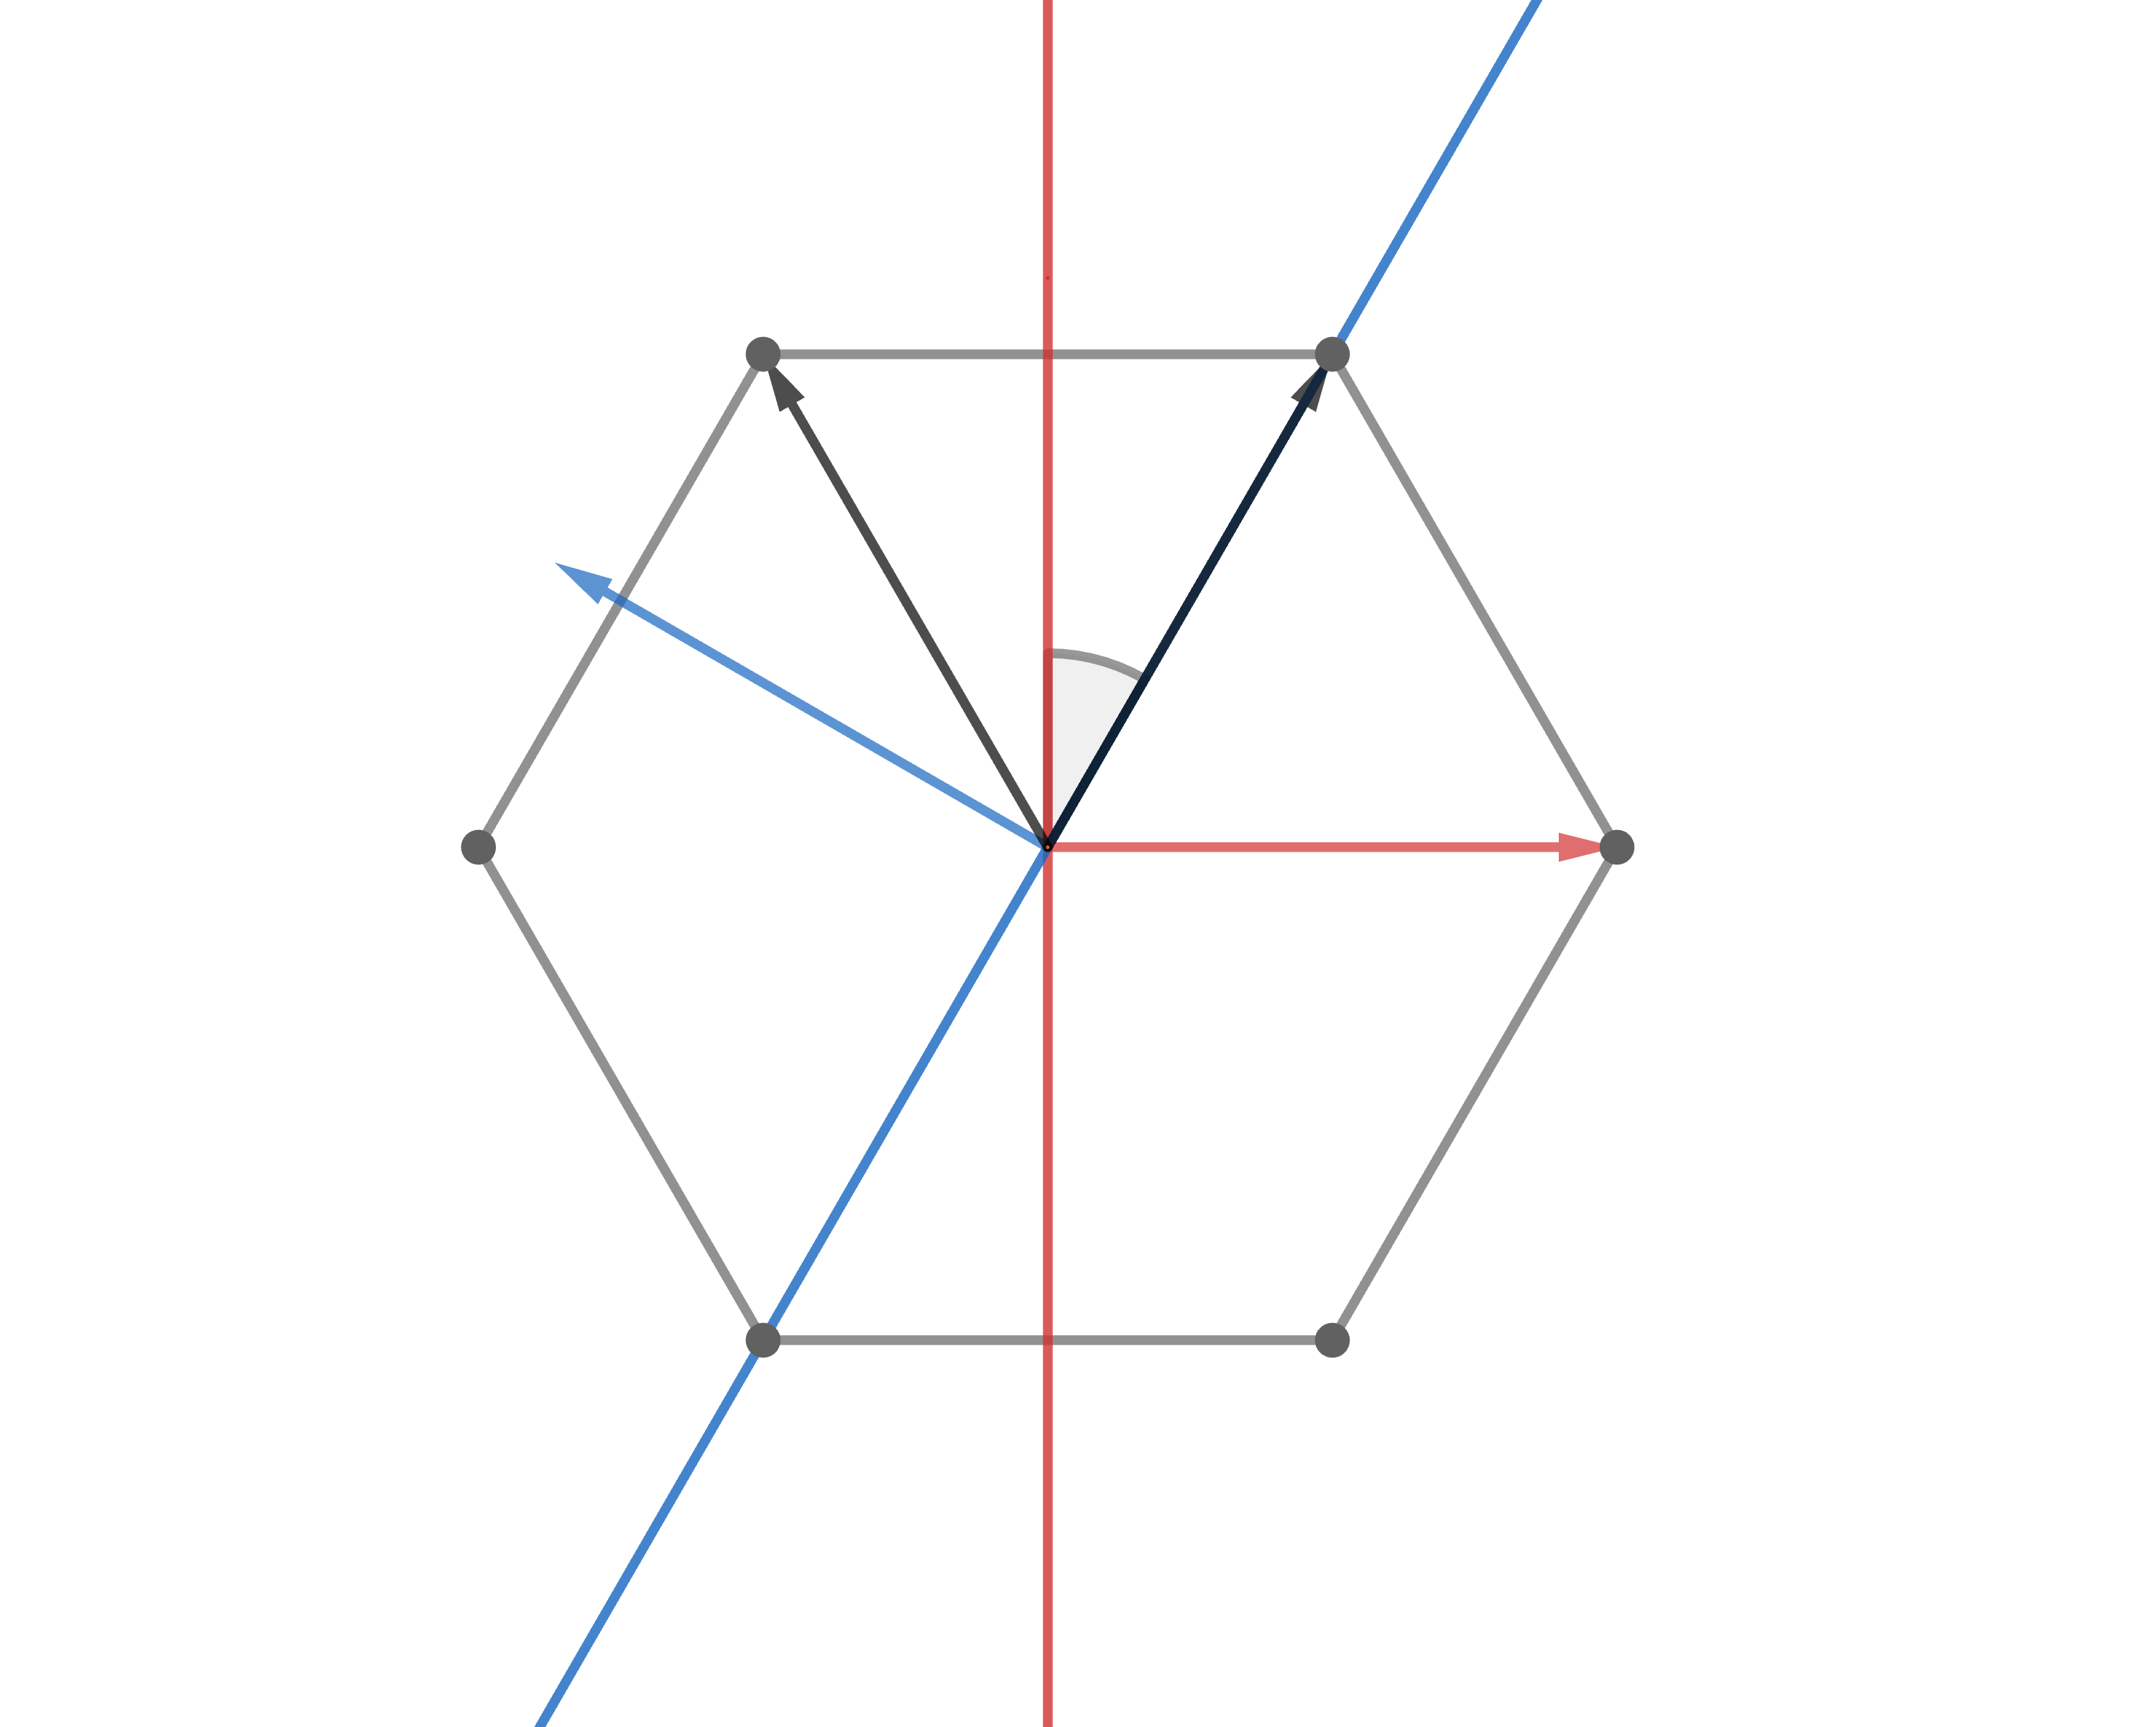
\includegraphics[width=5cm]{gfx/the dihedral proof case.png}
% \end{figure} % TODO: fix the image


% ***********************************************
\section{The fundamental domain and Stabilizers}
% ***********************************************

In this section, we will prove that the fundamental chamber \(C\subset V^*\) is indeed a fundamental domain for the action of \(W\) on its Tits cone \(WC\).
Moreover, we will work out how stabilizers of points look like and then show that the Tits cone is really a convex cone in the dual space \(V^*\).

We start by translating the results of the previous section to the language of chambers and halfspaces.
The following two lemmas capture this essence.

\begin{lemma}\label{lem:translation}
    Let \(w\in W\) and \(i\in I\).
    % Then the relation \(\ell(s_iw) > \ell(w)\) of \(s_i\) and \(w\) is equivalent to \(w(\mathring{C})\subset A_i^*\), \ie \(\;w\) leaving the open chamber inside the open halfspace, corresponding to \(s_i\).
    The relation \(\ell(s_i w) > \ell(w)\) is equivalent to saying that \(w\) leaves the open chamber \(\mathring{C}\) inside the open halfspace \(A_i^*\), corresponding to the generator \(s_i\).
    Put more formally, this states that the set \(w(\mathring{C})\) is a subset of the open halfspace \(A_i^*\).
\end{lemma}
\begin{proof}
    Observe that \(\ell(s_iw) > \ell(w)\) is equivalent to \(\ell(w^{-1}s_i) > \ell(w^{-1})\).
    Then by by \Cref{thm:action}, we have that \(w^{-1}(e_i) > 0\).
    Take an arbitrary point \(\varphi\in \mathring{C}\) in the open fundamental chamber, then we have that \(w(\varphi)(e_i) = \varphi(w^{-1}(e_i))\).
    Since the chamber \(C\) lies in \(A_i^*\) for all \(i\in I\) and \(\varphi \in \mathring{C}\), we see that \(w(\varphi) > 0\) is equivalent to \(w^{-1}(e_i)>0\).
    But this is true by assumption and since \(\varphi\) is arbitrary, we conclude that \(w(\mathring{C}) \subset A_i^*\).
\end{proof}

Of course this lemma also has a corresponding converse result as in the previous section.
% If we choose in the above lemma \(\widetilde{w} := s_iw\) for an \(i \in I\), we get
% \[\ell(s_i\widetilde{w}) = \ell(s_i^2 w) = \ell(w) > \ell(s_iw) = \ell(\widetilde{w}) \iff \widetilde{w}(C) = s_iw(C)\subset A_i^*.\]
% This is again equivalent to \(w(\mathring{C}) \subset s_i(A_i^*)\), and we have just proved the following lemma as the counterpart to \Cref{lem:translation}.

\begin{lemma}\label{lem:translation2}
    Let \(w\in W\) and \(i\in I\).
    % Then the relation \(\ell(s_iw) < \ell(w)\) holds if and only if we have \(w(\mathring{C})\subset s_i(A_i^*)\), \ie \(\;w\) moves the open chamber into the open halfspace complementary to \(A_i^*\).
    The relation \(\ell(s_i w) < \ell(w)\) is equivalent to saying that \(w\) now moves the open chamber \(\mathring{C}\) inside the open halfspace, complementary to \(A_i^*\).
    More formally, this states that the set \(w(\mathring{C})\) is a subset of the open halfspace \(s_i(A_i^*)\), as the \(s_i\) permute \(A_i^*\) and its corresponding complementary halfspace.
\end{lemma}
\begin{proof}
    Take \(w' = s_i w\) for some \(i \in I\) and \(w \in W\) so that \(\ell(s_i w) > \ell(w)\).
    Then we have that the length of \(s_i w' = w\) is strictly smaller then then length of \(w'\).
    % Then we have that \(\ell(s_i w') = \ell(w) < \ell(s_i w) = \ell(w')\)
    By applying above lemma we get that \(w(\mathring{C}) \subset A_i^*\), which is equivalent to \(s_i w'(\mathring{C}) \subset A_i^*\).
    Apply \(s_i\) to both sides leaves us with \(w'(\mathring{C}) \subset s_i(A_i^*)\), which proves the lemma.
\end{proof}

Building onto this insight, we now want to study the action of parabolic subgroups on the Tits cone to get an understanding of the stabilizers of points.
To do so, decompose the fundamental chamber into subsets corresponding to the parabolic subgroups of \(W\) as follows.

\begin{definition}
    Given a parabolic subgroup \(W_J\) corresponding to \(J\subset I\), set
    \[C_J := \bigcap_{j\in J} H_j^* \cap \bigcap_{k\notin J} A_k^*.\]
    We call these the corresponding parabolic subsets (of the fundamental chamber).
\end{definition}

\begin{example}\label{ex:parabolicset} % TODO: add picture
    \begin{enumerate}
        \item When the set \(J\) is empty, the corresponding parabolic subset \(C_\emptyset\) coincides with the entire chamber \(C\).
              Conversely, when \(J\) contains all indices, \(C_J\) reduces to the singleton \(\{0\}\).
        \item If \(J\) is a proper subset of \(I\) with cardinality one, then the corresponding subset \(C_J\) coincides with a codimension-one face of the chamber \(C\).
    \end{enumerate}
\end{example}

\begin{theorem}\label{thm:stabilizer}
    Let \(w\in W\) and \(J, K \subset I\) be subsets.
    Then \(w(C_J)\cap C_K \neq \emptyset\) implies \(J = K\), \(w\in W_J\) and thus \(w(C_J) = C_J\).
    In particular, the isotropy groups of the sets \(C_J\) are the parabolic subgroups \(W_J\).
\end{theorem}
\begin{proof}
    Let \(w\in W\) and \(J, K\subset I\) be subsets, such that \(w(C_J)\cap C_K \neq \emptyset\).
    % We also proof this theorem by induction on \(\ell(w)\), with the base case \(\ell(w) = 0\) being trivial.
    The proof is by induction on the length of \(w\).
    The base case \(\ell(w) = 0\) is trivial, as then \(w\) is trivial.

    Assume that \(\ell(w) > 0\) and choose \(i\in I\), such that \(\ell(s_iw) < \ell(w)\).
    Writing \(w = s_i(s_iw)\), by \Cref{lem:translation2} we know that \(w\) moves the open chamber \(\mathring{C}\) into the open halfspace \(s_i(A_i^*)\), i.e. \(w(\mathring{C})\subset s_i(A_i^*)\).
    Now using the continuity of the group action, we note that \(w(C) \subset \overline{s_i(A_i^*)}\). %is a subset of \(\overline{s_i(A_i^*)}\).
    Recall that by definition, the fundamental chamber \(C\) lies in the halfspaces \(\overline{A_i^*}\) for all \(i \in I\).
    % Now we use the continuity of the action of \(W\) to get that \(w(C)\subset \overline{s_i(A_i^*)}\), which then implies that \(w(C)\cap C\subset H_i^*\).
    % This follows, since the (closed) fundamental chamber \(C\) by definition is a subset of \(\overline{A_i^*}\).
    Thus, we record that \(w(C) \cap C \subset H_i^*\) and since \(s_i\) fixes the corresponding \(H_i^*\) by definition, it fixes every point in the intersection of \(C\) and its translate \(w(C)\).
    Note that the sets \(C_J\) and \(C_K\) are subsets of the fundamental chamber \(C\) and therefore, \(s_i\) fixes every point in the non-empty set \(w(C_J)\cap C_K\).
    But if \(s_i\) fixes some point \(\varphi\) in \(C_K\), we calculate
    \[\varphi(e_i) = s_i(\varphi)(e_i) = \varphi(s_i(e_i)) = -\varphi(e_i) \implies \varphi(e_i) = 0 \iff \varphi\in H_i^*.\]
    We deduce \(i\in K\), respectively \(s_i\in W_K\).
    Using this together with the assumption, we get that \(s_iw(C_J)\cap C_K = s_i(w(C_J)\cap C_K)\) is non-empty.
    We apply the induction hypothesis to the element \(s_iw\), to see that \(J = K\) and \(s_iw\in W_J\).
    Finally, since \(s_i\in W_J = W_K\), we have that \(s_iw \in W_J\) implies \(w\in W_J\), proving the theorem.
\end{proof}

% For the next theorem we want to prove, we want to recall the following definition.
Before proceeding with proving that the fundamental chamber lives up to its name, we want to clearly state what is meant by a fundamental domain.

\begin{definition}
    Let \(G\) be a group, acting on a topological space \(X\).
    We call a closed subset \(F\subset X\) a \emph{(strict) fundamental domain}, if for each \(x\in F\) its orbit \(Orb(x)\) intersects \(F\) in exactly one point.
\end{definition}

Note that, by definition of the Tits cone \(WC\), every \(W\)-orbit of a point \(\varphi\in C\) meets the fundamental chamber \(C\) in at least one point, namely \(\varphi\).
Thus, it suffices to proof that each \(W\)-orbit meets \(C\) in at most one point, to prove the following theorem.

\begin{theorem}\label{thm:funddomain}
    The fundamental chamber is a fundamental domain for the action of the Coxeter group \(W\) on its Tits cone \(WC\), justifying its name.
\end{theorem}
\begin{proof}
    Assume that \(\varphi,\psi\in C\) lie in the same \(W\)-orbit, but in different parabolic subsets \(C_J\), respectively \(C_K\) of the fundamental chamber. %, for \(J,K\subset I\).
    Since they lie in the same orbit, there is a \(w\in W\) with \(\varphi = w(\psi)\).
    Thus, the intersection \(w(C_J)\cap C_K\) is non-empty and \Cref{thm:stabilizer} implies equality of \(J\) and \(K\), as well as \(w \in W_J\).
    We deduce \(\varphi = w(\psi) = \psi\).
    Thus, every \(W\)-orbit of a point \(\varphi\in C\) meets the fundamental chamber \(C\) at most in \(\varphi\), proving the theorem.
\end{proof}

Define a set \(\mathcal{C}\) as the union of all translates of possible parabolic subsets \(C_J\) \ie, define \(\mathcal{C}\) by
\[\mathcal{C} := \bigcup_{J \subset I} \bigcup_{w \in W/W_J} w(C_J).\]
We want to emphasize here that by \Cref{thm:stabilizer} the sets of the form \(w(C_J)\) in the Tits cone \(WC\) are all disjoint for different \(J \subset I\) and \(w\) ranging over the coset \(W/W_J\).
% Note that \Cref{thm:stabilizer} implies that this set forms a partition of the Tits cone as it shows that the sets of the form \(w(C_J)\) in \(\mathcal{C}\) are all disjoint for \(w\) in the coset \(W/W_J\) and \(J\) a subset of \(I\).
Thus, the sets of \(\mathcal{C}\) form a partition of the Tits cone.
This decomposition (altough not into chambers) is a key component in the following theorem.

\begin{theorem}\label{thm:convexity}
    The Tits cone \(WC\) is a convex cone, and every closed line segment in the Tits cone meets only finitely many of the sets in \(\mathcal{C}\).
\end{theorem}
\begin{proof}
    First note that the fundamental chamber is a convex cone as the intersection of the finitely many closed halfspaces \(\overline{A_i^*}\).
    This implies that the Tits cone is a cone as well.
    We will prove the convexity by showing that every closed segment between any two points in the Tits cone is contained in it.
    Furthermore, we will prove that these segments can be covered by finitely many of the sets in the above defined union \(\mathcal{C}\), implying latter statement.

    Consider the closed segment \([\varphi, \psi]\) with \(\varphi, \psi \in WC\) and assume the endpoints lie in different chambers. % \(\varphi\in C\) and \(\psi\in w(C)\) for some \(w\in W\), i.e. the endpoints lie in different chambers.
    Proceed by induction on the word length \(\ell(w)\). %with the base case \(\ell(w) = 0\) implying \(\varphi,\psi\in C\).
    The base case \(\ell(w) = 0\) reduces to \(\varphi, \psi \in C\).
    Since \(C\) is convex and can trivially be covered by finitely many of the \(C_J\), this case has been dealt with.
    
    Therefore, we now assume \(\ell(w) > 0\).
    Intersect the segment \([\varphi, \psi]\) with the fundamental chamber \(C\), to receive two new segments \([\varphi, \xi]\) and \([\xi, \psi]\) (cf. \Cref{img:path}).
    % Note that we can divide the segment \([\varphi, \psi]\) into two parts, by intersecting it with the closed chamber \(C\) to get a closed segment \([\varphi, \xi]\) inside \(C\) and a segment \([\xi, \psi]\).
    The first segment can be covered by finitely many of the sets in \(\mathcal{C}\), as it lies inside the fundamental chamber \(C\).
    Thus, we need to show that we can cover the second segment \([\xi, \psi]\) by finitely many of these sets.
    Assume further, we have a \(J \subset I\), such that \(\psi\in s_i(A_i^*)\) for an \(i\in J\) and \(\psi\in\overline{A_i^*}\) for all \(i\notin J\).
    Then we have that \(\psi\notin C\).
    \Claim{1}{\(\xi\) has to lie in one of the codimension-one faces \(H_i^*\), \(i\in J\).}
    \Claimproof{1}{
        Assume that \(\xi\) lies in the open halfspace \(A_i^*\) for some \(i\in J\).
        Then every point \(\zeta\) in the intersection of a neighborhood of \(\xi\), contained in \(A_i^*\), with the segment \([\xi,\psi]\) has to also lie in \(A_i^*\). % for \(i\in J\). % and \(\zeta\in \overline{A_i^*}\) for \(i\notin J\).
        Clearly, \(\zeta\in\overline{A_i^*}\) for \(i\notin J\) holds as well, implying that \(\zeta\in C\).
        But this is a contradiction to the decomposition of the initial segment \([\varphi, \psi]\).
        Thus, \(\xi\) has to lie in one of the \(H_i^*\).
    }
    Using the assumptions \(\psi\in s_i(A_i^*)\) and \(\psi\in w(C)\), we deduce \(w(C)\subset \overline{s_i(A_i^*)}\), hence by continuity of the action \(w(\mathring{C})\subset s_i(A_i^*)\).
    By \Cref{lem:translation2} this is equivalent to \(\ell(s_iw) < \ell(w)\) and we are set up to apply the induction hypothesis to \(\xi\) and \(s_i(\psi)\in s_iw(C)\).
    This produces a cover of \([\xi,s_i(\psi)]\) by finitely many sets in \(\mathcal{C}\).
    But since we established that \(\xi\) has to lie in \(H_i^*\), translation by \(s_i\) gives \([s_i(\xi), s_i^2(\psi)] = [\xi, \psi]\), and thus we can cover this segment by finitely many sets as well.
    The result follows.
\end{proof}

\begin{figure}[ht]
    \centering
    \subfloat[\centering A path through the Tits cone.]{{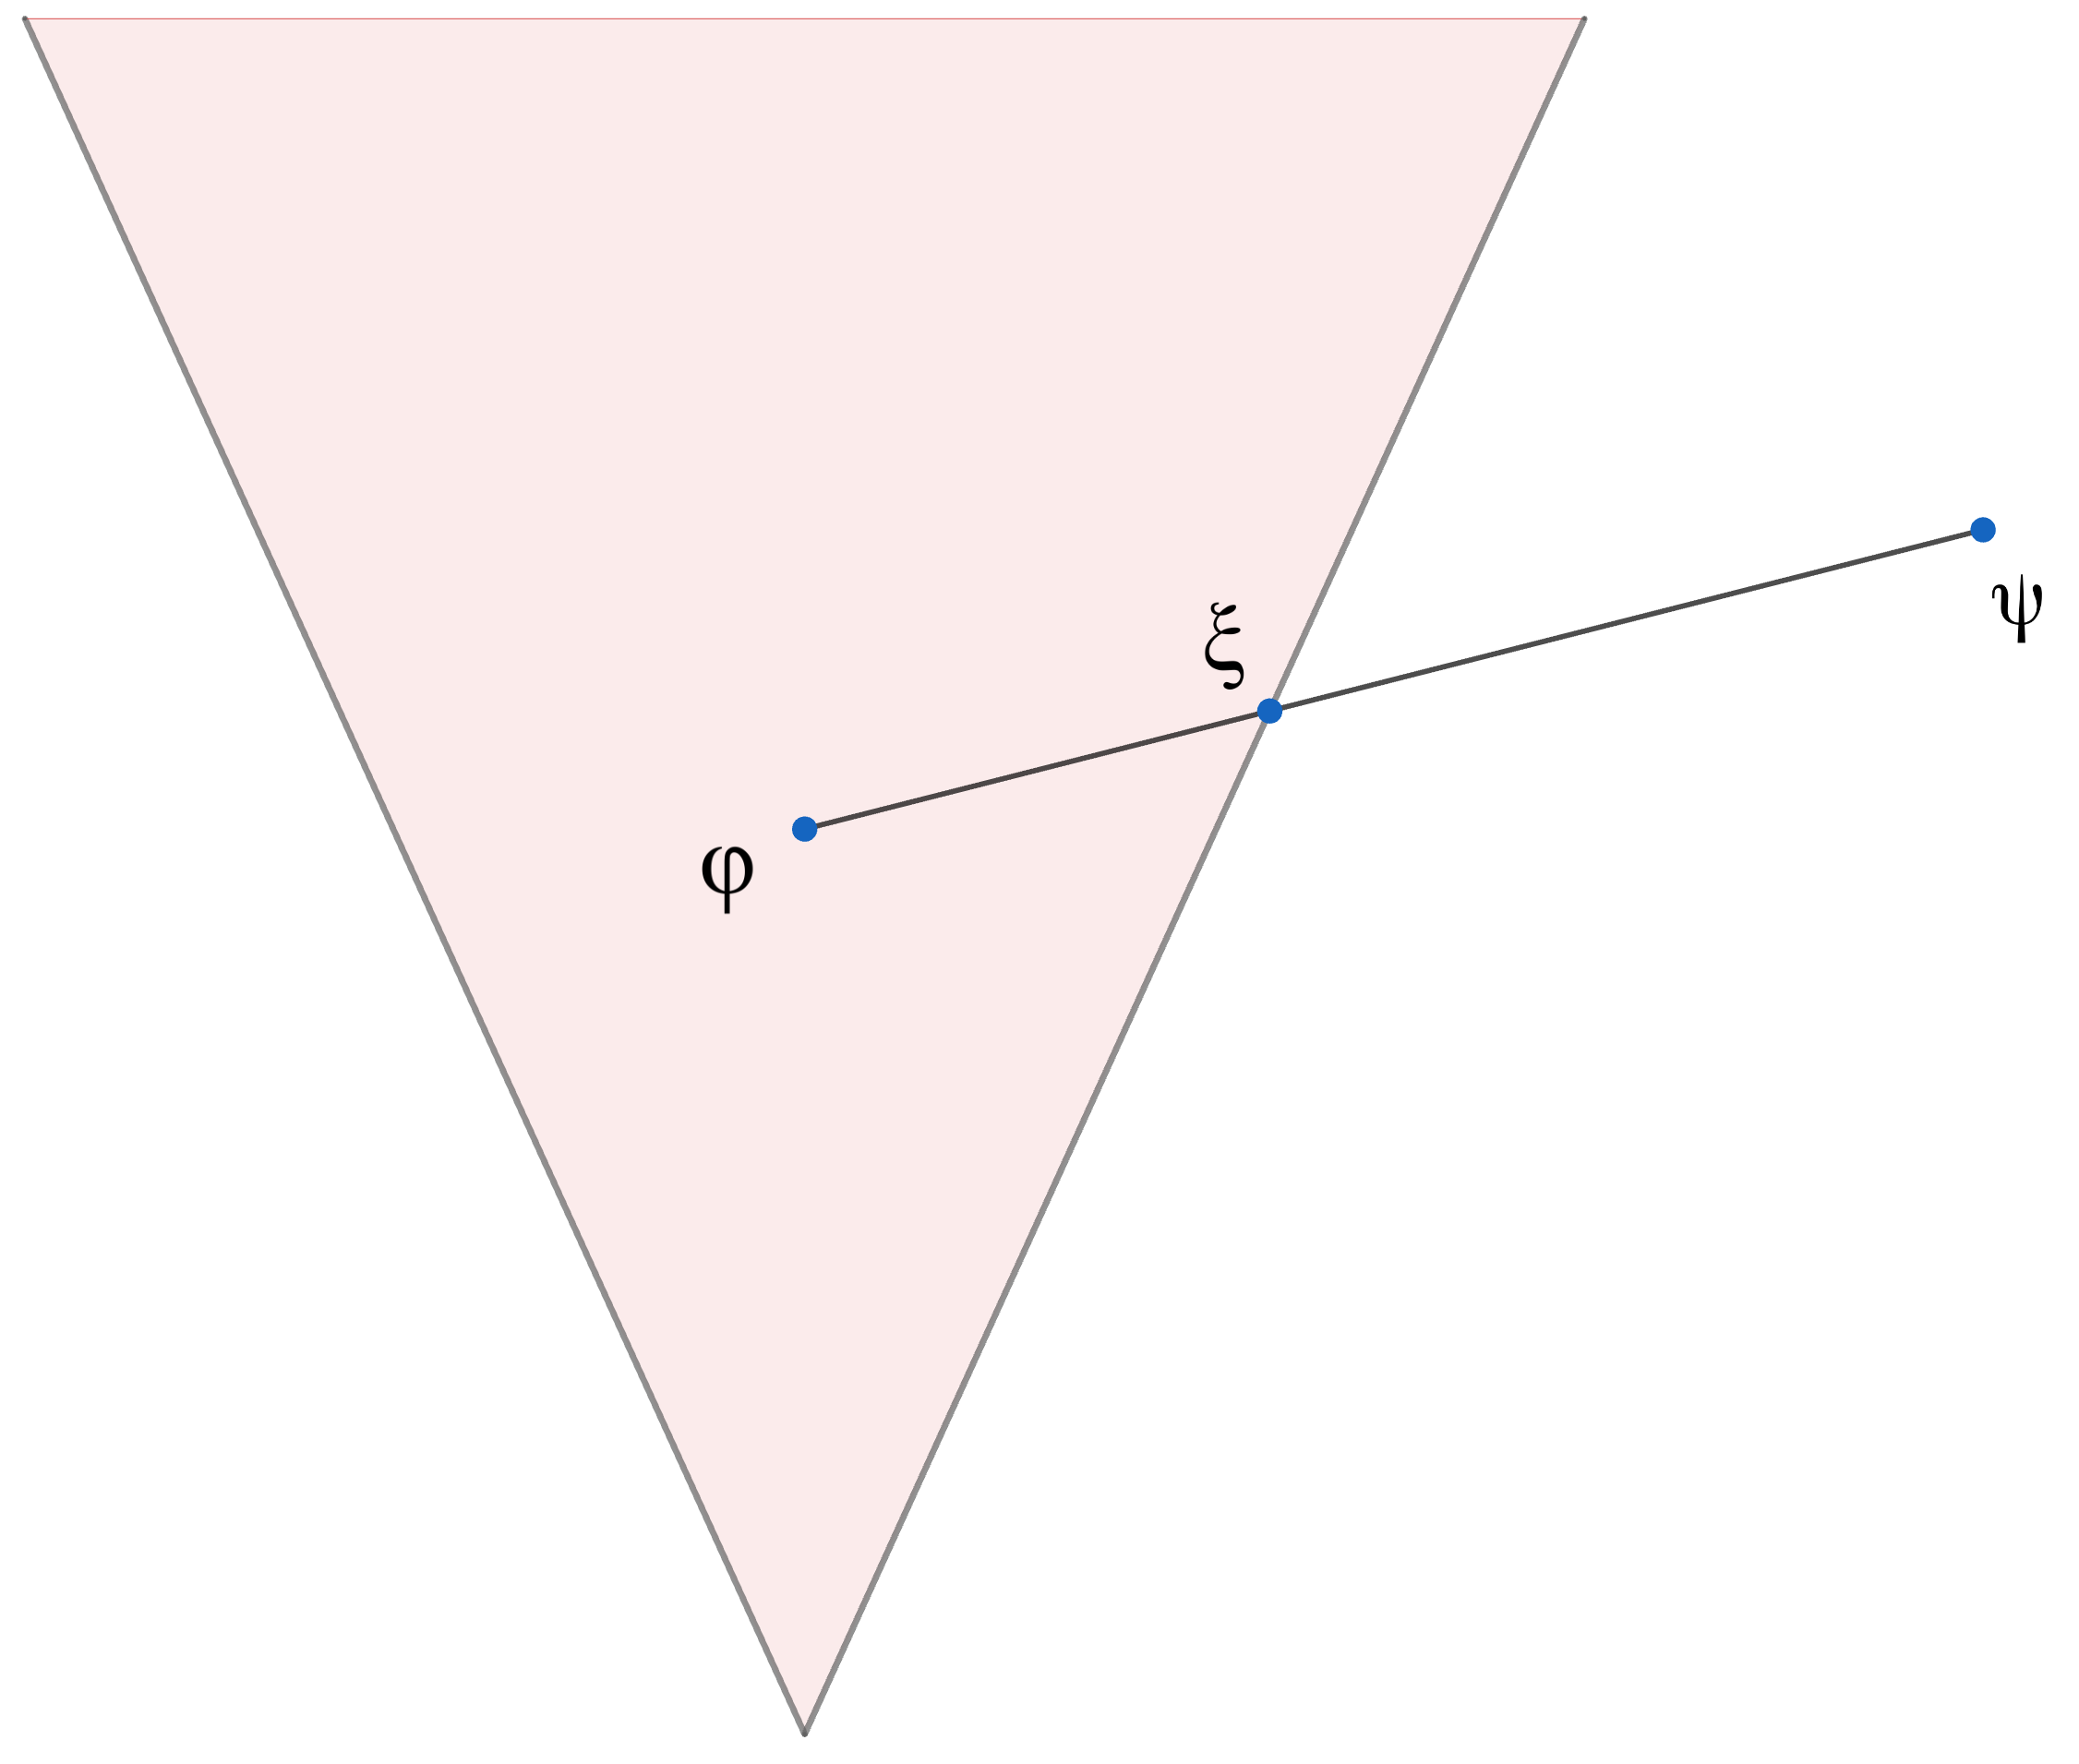
\includegraphics[width=5cm]{gfx/pfad durch kegel.png}}\label{img:path}}
    \qquad
    \subfloat[\centering A neighborhood of \(\xi\).]{{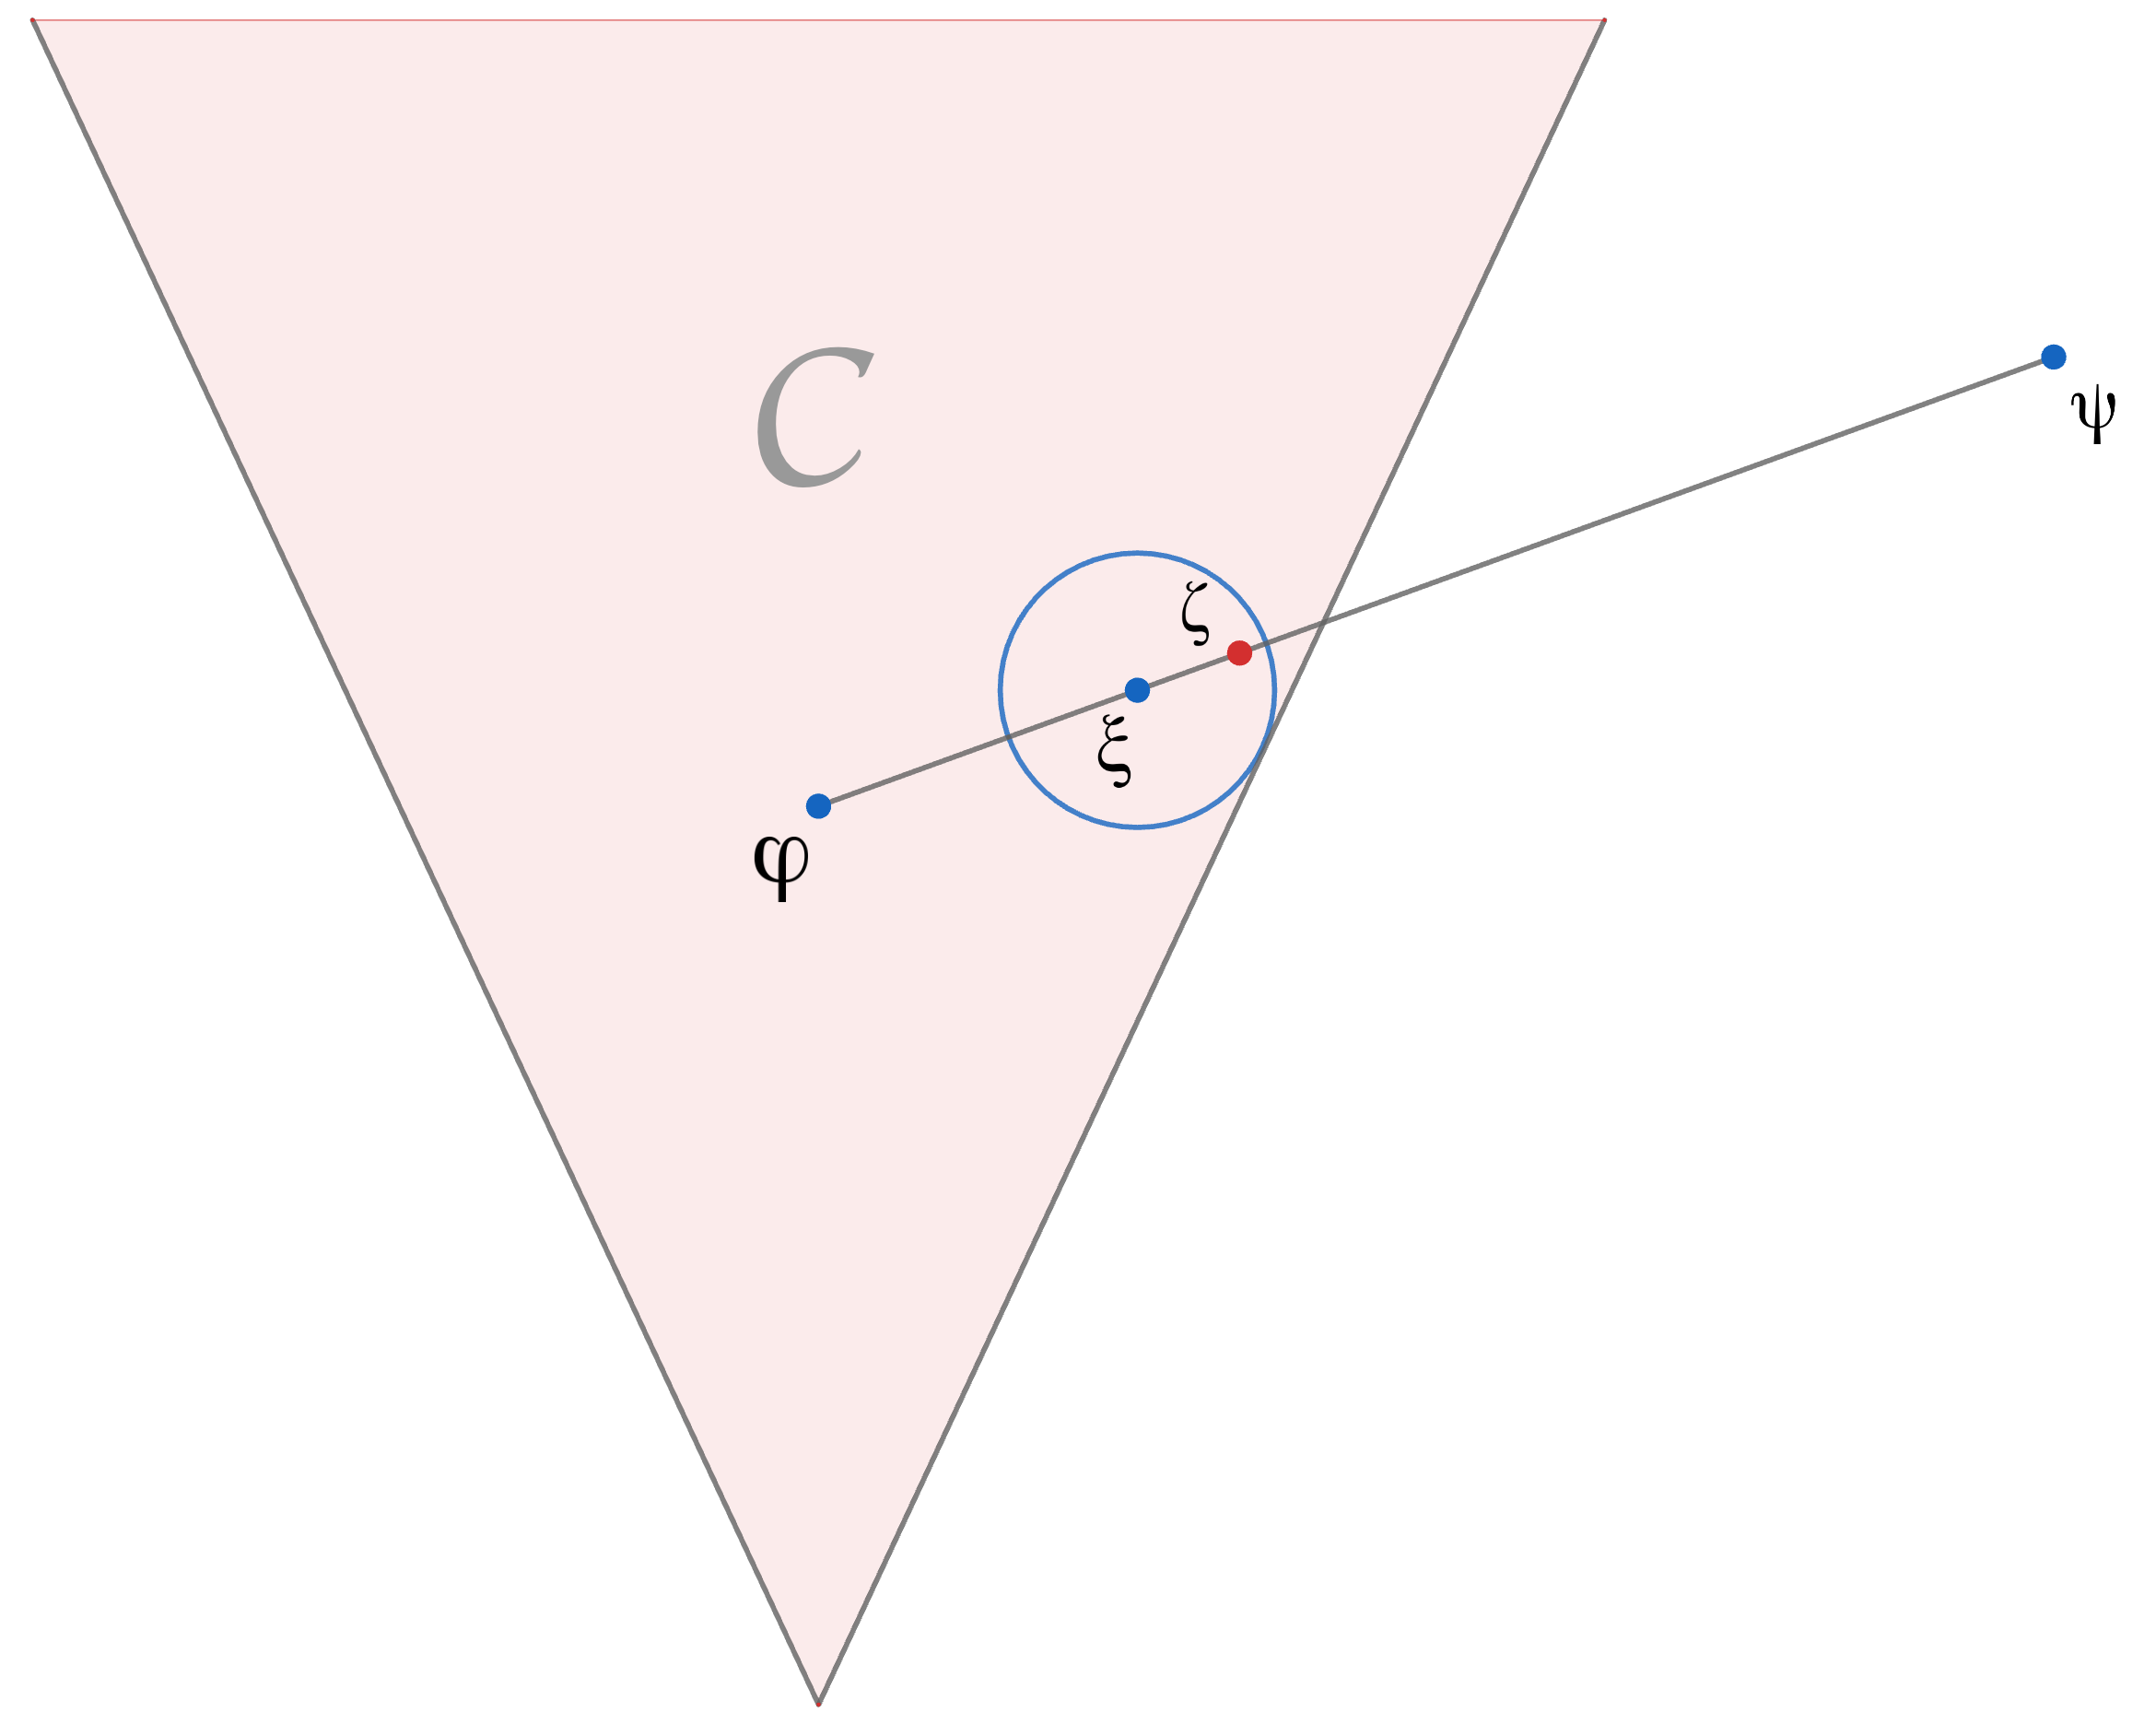
\includegraphics[width=5.35cm]{gfx/the neighborhood.png}}}
    % \caption{The picture to the proof.}
\end{figure}

To summarize, the essence of this section is that first of all the fundamental chamber is indeed a fundamental domain of the action of a Coxeter group on its Tits cone.
This was shown in \Cref{thm:funddomain}.
Furthermore, we want to emphasize that each point in the interior of the fundamental chamber has trivial stabilizer, which is a direct consequence of \Cref{thm:stabilizer}.
Moreover, every point in a parabolic subset \(C_J\) of \(C\), for \(J\) a subset of \(I\), is stabilized by the corresponding parabolic subgroup \(W_J\).

% An essential fact we want to emphasize here is that the stabilizer of the fundamental chamber is trivial.
% Setting \(J=K=\emptyset\), we obtain from \Cref{thm:stabilizer} (using that \(C_\emptyset = C\)), that if \(wC\cap C \neq \emptyset\) we must have \(w\in W_\emptyset = \{1\}\).
% Setting \(J=\emptyset\), we obtain from \Cref{thm:stabilizer} that the stabilizer subgroup of \(C_J = C_\emptyset = C\) (cf. \Cref{ex:parabolicset}) is precisely the parabolic subgroup \(W_J = W_\emptyset = \{1\}\).


% ***********************************************
\section{Covering actions - A Toolbox}
% ***********************************************

In this section we will assemble a set of tools, mostly coming from algebraic topology, connecting group actions to the notion of coverings.
They will be somewhat essential in the proof of the main theorem in the next chapter.
We start by saying what is meant by a covering.

\begin{definition}\label{def:covering}
    Let \(X, Y\) be topological spaces.
    A continuous map \(p: Y\to X\) is a \emph{covering map} and \(Y\) a \emph{covering space} for \(X\), if every point \(x\) in \(X\) has an open neighborhood \(U\), such that the preimage of \(U\) under \(p\) is a disjoint union of open sets \(U_i\) in \(Y\) for an index set \(I\).
    Furthermore, the map \(p\) has to be a local homeomorphism, meaning the restriction of \(p\) to the \(U_i\) is a homeomorphism onto its image \(p(U_i)\).
    Then, \(U\) is called \emph{evenly covered} and \(\vert I \vert\) the degree of the covering, while the open sets \(U_i\) are called the \emph{sheets} over \(U\) and the preimage of an \(x\) in \(X\) is called a \emph{fiber} of \(x\).
\end{definition}

It turns out that restricting the action of a group on a topological space in the right way will give coverings by quotienting out the action.
We make this precise in the following.

\begin{definition}
    Let \(G\) be a group, acting on a space \(X\).
    The action is said to be \emph{properly discontinuous}, if every point in \(X\) has a neighborhood \(U\) such that the set \(\{g\in G\;\vert\; g(U)\cap U \neq \emptyset\}\) is finite.
\end{definition}

\begin{definition}
    Let \(G\) be a group, acting on a space \(X\).
    The action is said to be a \emph{covering (space) action} if every point has a neighborhood \(U\) such that the set \(\{g\in G \;\vert\; g(U)\cap U \neq \emptyset\}\) consists only of the neutral element.
\end{definition}

Obviously, this last condition is even more restrictive.
Yet, at least for Hausdorff spaces, there is a connection between the two.
In addition to acting properly discontinuously, we have to demand the action to be free.

\begin{lemma}
    Let \(G\) be a group that acts freely and properly discontinuously on a Hausdorff space \(X\).
    Then the action of \(G\) is a covering action in the above sense.
\end{lemma}
\begin{proof}
    Let \(X\) be a Hausdorff space and \(G\) be a group acting freely, properly discontinuously on \(X\).
    Then for an open neighborhood \(U\) of \(x\in X\), the set \(M := \{g \in G \;\vert\; gU \cap U \neq \emptyset\}\) is finite.
    For these \(g \in M\) we pick pairwise disjoint Neighborhoods \(V_g\) of \(gx\), which is possible since \(X\) is Hausdorff and \(G\) acts freely (thus \(gx \neq x\)).
    Finally, set \(V = \left(\bigcap_{g \in M} g^{-1} V_g \right) \cap U\), which is open as finite intersection of open sets and by definition a neighborhood of \(x\).
\end{proof}

To finally construct coverings from group actions and connect them in some sense, we need a last condition on the space the group acts on.

\begin{definition}
    A path-connected topological space \(X\) is called \emph{simply connected}, if \(\pi_1(X)\cong \{1\}\).
\end{definition}

\begin{lemma}\label{lem:covering}
    Let \(G\) be a group, acting by a covering action on a simply connected topological space \(X\).
    Then the quotient map \(p_G:(X, x_0)\to (G\backslash X, Orb(x_0))\) is a covering map and \(\pi_1(G\backslash X, Orb(x_0))\cong G\).
\end{lemma}
\begin{proof}
    Let \(U\) be an open neighborhood of \(x\in X\), such that \(\{g \in G \;\vert\; gU \cap U \neq \emptyset\} = \{1\}\).
    \Claim{1}{The map \(p_G\) restricted to \(U\) is a continuous bijection onto its image \(p_G(U)\).}
    \Claimproof{1}{
        \begin{itemize}
            \item Continuity: \(V\subset G\backslash X\) is open if and only if \(p_G^{-1}(V)\) is open and thus \(p_G\) is continuous.
            \item Surjectivity: Since orbits of points are non-empty, \(p_G\) is surjective.
            \item Injectivity: Assume \(x,y \in X\) distinct with \(p_G(x) = p_G(y)\).
                But then there is a non-trivial element \(g \in G,\; g \neq 1_G\) with \(gx = y\), implying \(g(U) \cap U \neq \emptyset\).
                This is a contradiction to \(G\) acting by a covering action.
        \end{itemize}\vspace*{-2\parskip}
    }\vspace*{-2\parskip}
    \Claim{2}{Every point \(Orb(x) \in G\backslash X\) has a neighborhood \(V \subset G \backslash X\) with \(p_G^{-1}(V) = \bigsqcup_{g \in G} gU\).}
    % \Claim{2}{Every point \(Orb(x) \in G\backslash X\) has a neighborhood \(V := p_G(U)\), \(U\) as in \emph{Claim 1}, hence \(p_G^{-1}(V) = \bigsqcup_{g \in G} gU\).}
    \Claimproof{2}{
        By assumption the sets \(gU\) are all disjoint neighborhoods of \(gx \in X\) for all \(g \in G\).
        Moreover, for \(V := p_G(U) \subset G\backslash X\), we have \(p_G^{-1}(V) = \bigsqcup_{g \in G} gU\), proving the Claim.
    }\vspace*{-2\parskip}
    \Claim{3}{The map \(p_G\vert_{gU} \to V = p_G(U)\) is a homeomorphism for all \(g \in G\).}
    \Claimproof{3}{
        Note that the action of \(G\) on \(X\) is by homeomorphisms and \(U \subset X\) is open.
        Then the union \(\bigsqcup_{g \in G} gU\) is open as well and since \(p_G^{-1}(V) = \bigsqcup_{g \in G} gU\), the set \(V\) is open in the quotient topology of \(G \backslash X\).
        Therefore, the map \(p_G\) restricted to \(gU\) for \(g \in G\) is an open map and hence, by \emph{Claim 1} a homeomorphism.
    }
    Now all conditions in \Cref{def:covering} are satisfied, so \(p_G\) is a covering map.
    For the last part of the statement, note that \(X\) is simply connected, implying that it is the universal cover of \(G \backslash X\). %\(\faktor{X}{G}\).
    By definition, \(G\) is the group of Deck transformations, thus \(\pi_1(G \backslash X, Orb(x_0)) \cong G\).
    % For the last part of the statement, take a homotopy class of loops \([\gamma] \in \pi_1(G \backslash X, Gx_0)\) with representative \(\gamma\).
    % Define a map \(\varphi : \pi_1(G, x_0) \to G\) on homotopy classes \([\gamma]\), such that \(\varphi([\gamma])\) takes \(\widetilde{\gamma}(0) = x_0\) to \(\widetilde{\gamma}(1)\), where \(\widetilde{\gamma}: [0,1] \to X\) is a lift of \(\gamma\).
    % Now if \(\gamma'\) is another representative of \([\gamma]\) then, \(\widetilde{\overline{\gamma}'\cdot \gamma}\) is the lift of a contractible curve in \(G \backslash X\).
\end{proof}
